\documentclass[a4,12pt]{article}

%%%%%%%%%%%%%%%%%%%%%%%%%%%%%%%%%%%%%%%%%%%%%%%%%%%%%%%%%%%%%%%%%%%%%%%%%%%
%                             REQUIRED PACKAGES
%%%%%%%%%%%%%%%%%%%%%%%%%%%%%%%%%%%%%%%%%%%%%%%%%%%%%%%%%%%%%%%%%%%%%%%%%%%
\usepackage[latin1]{inputenc}
\usepackage[affil-it]{authblk}
\usepackage{amsmath, amsfonts, amssymb, bm, bbm} % Math packages
\usepackage{pifont}
\usepackage{graphicx}
\usepackage[ocgcolorlinks]{hyperref}
\usepackage{titlesec}
\usepackage[table]{xcolor}
\usepackage{multirow}
\usepackage{booktabs}
\usepackage{vwcol}
\usepackage[labelfont={small,bf}, textfont={small}, labelsep=space, tableposition=top]{caption}
\usepackage{subcaption}
\captionsetup[subfigure]{font=scriptsize,labelfont=scriptsize}
\usepackage[ruled,linesnumbered,vlined]{algorithm2e}
\usepackage{minted}    
\usemintedstyle{VS}
\usepackage[title]{appendix}
\usepackage[numbers]{natbib}
\bibliographystyle{IEEEtranN}
%\bibpunct{(}{)}{;}{a}{,}{,}
\usepackage{multicol}

\usepackage{pgf,tikz,pgfplots,calc}
\usetikzlibrary[calc]
\usetikzlibrary{positioning}
\pgfplotsset{compat=1.15}
\usepackage{mathrsfs}
\usepackage{relsize}

%%%%%%%%%%%%%%%%%%%%%%%%%%%%%%%%%%%%%%%%%%%%%%%%%%%%%%%%%%%%%%%%%%%%%%%%%%%
\usepackage{jour} % style

\title{\bfseries Factorizer: A Scalable Interpretable Approach to Context Modeling for Medical Image Segmentation}
\author[a]{\normalsize Pooya Ashtari \footnote{Corresponding author. Email: \url{pooya.ashtari@esat.kuleuven.be}}}
\author[a]{\normalsize Sabine Van Huffel}

\affil[a]{\footnotesize Department of Electrical Engineering (ESAT), KU Leuven}

\date{}

\begin{document}
	\maketitle
	
	\begin{abstract}
		Medical image segmentation is crucial for various clinical purposes. The vast majority of state-of-the-art segmentation models are Convolutional Neural Networks (CNNs) comprising encoder and decoder paths with skip connections in between. However, the inherent locality of convolution makes these models fail to effectively exploit long-range spatial dependencies, essential for better recognition of some structures, e.g., brain lesions. Transformers have recently proved promising performance on vision tasks, including semantic segmentation, mostly due to their capability of modeling global contexts. Nevertheless, lack of locality inductive bias makes Transformers underperform their CNN counterparts in low-data regimes, which is usually the case in medical imaging. Moreover, the quadratic complexity of attention makes exiting Transformer-based models use self-attention layers only after somehow reducing the image resolution, thus fail to fully exploit global contexts present at higher resolutions. Hence, this work introduces a family of models, dubbed Factorizer, which leverage the power of low-rank matrix factorization for constructing an end-to-end segmentation model. Specifically, we propose a linearly scalable approach to context modeling by formulating Nonnegative Matrix Factorization (NMF) as a differentiable layer integrated into a U-shaped architecture. The shifted window technique is also utilized in combination with NMF to effectively aggregate local information. Built upon matrix factorization, Factorizers compete favorably with CNNs and Transformers in terms of accuracy, scalability, and interpretability, achieving state-of-the-art results on the BraTS dataset for brain tumor segmentation. Highly meaningful NMF components give a great interpretability advantage to Factorizers over CNNs and Transformers. Moreover, our ablation studies reveal an interesting distinctive feature of Factorizers that enables a significant speed-up in inference for a trained Factorizer with no extra steps and without sacrificing much accuracy.	
		
		\vspace{4pt}\noindent Code: \url{https://github.com/pashtari/factorizer}
		\vspace{4pt}
	\end{abstract}
	
	\begin{keywords}
		Medical image segmentation, low-rank matrix factorization, convolution-free model.
	\end{keywords}
	
	\section{Introduction} \label{sec: introduction}
	
	Medical image segmentation is an essential prerequisite for the analysis of anatomical structures and various clinical purposes, including diagnosis and treatment planning. The vast majority of effective segmentation models are based on Convolutional Neural Networks (CNNs). In particular, U-Net \citep{ronneberger2015u}, consists of encoder and decoder parts with skip connections in between, has state-of-the-art performance on various medical image segmentation benchmarks. In a typical U-Net \citep{ronneberger2015u, cciccek20163d}, the encoder learns low-resolution contextual representation by progressively downsampling feature maps, while the decoder progressively upsamples the low-resolution feature maps to propagate contextual information to the higher-resolution layers. Moreover, skip connections from encoder layers to those of decoder at equal resolutions helps recover spatial information lost during downsampling.
	
	Currently, proposed U-Net models mostly rely on convolution operations with small receptive fields, which are capable of exploiting only local context at each resolution. Hence, they generally fail to effectively model long-range spatial dependencies, often necessary for better recognition of some region semantics, e.g., tumors with variable shapes and sizes. Several works \citep{chen2017deeplab, gu2019net} have employed dilated convolution for expanding the receptive fields. Nevertheless, the learning capabilities of convolutional layers are still limited due to their inherent locality. As a solution, integrating self-attention modules into CNNs \citep{wang2018non, fu2019dual} has been proposed to enhance the capability of modeling non-local context.
	
	Transformers \cite{vaswani2017attention} have achieved state-of-the-art performance on various Natural Language Processing (NLP) tasks. The attention mechanism enables Transformers to effectively model the pairwise interactions between the words in a sentence. Recently, Transformer-based models have been applied to vision tasks and proved promising. Specifically, Vision Transformer (ViT) \citep{dosovitskiy2020image} outperformed state-of-the-art CNNs on image recognition by large-scale pre-training and fine-tuning a pure Transformer. Unlike CNNs, ViT encodes images as a sequence of 1D patch embeddings (known as tokens) and dynamically highlights the important tokens using self-attention layers, which in turn increases the capability of learning long-range dependencies. Due to lack of locality inductive bias, ViT is data-hungry and generally requires a larger dataset to perform as effectively as its CNN counterparts, leading to poor performance when trained on insufficient data, which is usually the case in medical imaging. Furthermore, the quadratic complexity of self-attention makes Transformers computationally intractable on long sequences of patches. Therefore, exiting models use self-attention layers only after somehow reducing the image resolution, thereby failing to fully exploit the global context at the higher resolutions.  
	
	This work proposes a series of architectures, dubbed as Factorizer, which leverage the power of low-rank matrix factorization to construct an end-to-end medical image segmentation model. To this end, a linearly scalable alternative to self-attention is proposed by formulating a Nonnegative Matrix Factorization (NMF) algorithm as a differentiable layer. Moreover, a series of matricization operations are introduced, which enable NMF to effectively exploit both global and local contexts. The Factorizer block is constructed by replacing the self-attention layer of a ViT block with our NMF-based modules and then integrated into a U-shaped architecture with skip connections.
	
	We evaluate the effectiveness of our approach on the task of brain tumor segmentation in MRI data. Factorizes achieve competitive results on the BraTS dataset \citep{brats1, brats2, brats3} and outperform state-of-the-art methods based CNN and Transformer. Our experiments show that NMF components are highly meaningful, which gives a great advantage to Factorizers over CNNs and Transformers in terms of interpretability. Furthermore, our ablation studies reveal a distinctive interesting feature of Factorizers that enables us to easily speed up the inference for a trained Factorizer model with no extra steps and without sacrificing much accuracy.
	
	
	\paragraph{Contributions.}
	The main contributions of this work are as follows:
	\begin{itemize}
		\item To the best of our knowledge, this work presents the first end-to-end deep model with matrix factorization layers for medical image segmentation.
		\item We propose scalable interpretable U-Net-like models based on NMF for medical image segmentation. 
		\item We construct a differentiable layer performing NMF with a block coordinate descent solver to efficiently model contextual information. 
		\item Shifted Window (Swin) Matricize operation is proposed and combined with NMF to effectively exploit local contexts.
		\item The proposed models achieve state-of-the-art results on the BraTS dataset.
	\end{itemize}
	
	
	\paragraph{Notation.} Lets briefly overview notation. We denote vectors by boldface lower-case letters, e.g., $ \mathbf{x} $, matrices by boldface upper-case letters, e.g., $ \mathbf{X} $, and tensors by boldface calligraphic letters, e.g., $ \bm{\mathcal{X}} $. Elements in
	a matrix (tensor) are denoted by $ \mathbf{X}[i,j] $ ($ \bm{\mathcal{X}}[i_1, \dots, i_N] $). The $ i $th row and $ j $th column of a matrix is denoted by $ \mathbf{X}[i,:] $ and $ \mathbf{X}[:,j] $, respectively. A sequence of $ N $ vectors (a.k.a \textit{tokens}) is denoted by $ (\mathbf{x}_n)_{n=1}^{N} $. We use $ [\mathbf{x}_1|\dots|\mathbf{x}_N] $ to denote a matrix $ \mathbf{X} $ created by stacking $ \mathbf{x}_i $s along the columns. We show the inner product between matrices by $ \langle \mathbf{X}, \mathbf{Y} \rangle = \sum_{i,j} \mathbf{X}[i,j] \mathbf{Y}[i,j] $ and $ \ell _{2} $-norm of a matrix by $ \| \mathbf{X} \| = \sqrt{\langle \mathbf{X}, \mathbf{X}  \rangle} $.
	
	
	
	
	
	
	\section{Related Work} \label{sec: background}
	\paragraph{CNN-based Segmentation Models.}
	
	Convolution neural networks (CNNs) have dominated medical image segmentation. Particularly, following an encoder-decoder architecture with skip connections, U-Net \citep{ronneberger2015u} has achieved state-of-the-art on various medical image datasets. The simplicity and effectiveness of U-shaped architecture have made numerous U-Net variants
	emerge into the field. \citet{cciccek20163d} extended U-Net by replacing all 2D operations with their 3D counterparts. UNet++ \citep{zhou2018unet++} follows a deeply-supervised encoder-decoder network consisting of sub-networks connected through a series of nested, dense skip connections. nnU-Net \citep{isensee2021nnu} proved effective in various medical image segmentation tasks by only making minor modifications to the standard 3D U-Net \citep{cciccek20163d} and defining a recipe to automatically configure key design choices. \citet{myronenko20183d} proposed a U-Net-like architecture with ResNet blocks, a.k.a ResSegNet, winning first place in the Brain Tumor Segmentation Challenge (BraTS) 2018.
	
	Despite their success, these networks generally fail to effectively model long-range spatial dependencies, often necessary for better recognition of some region semantics such as tumors, since they rely on convolution operations with small kernel sizes, aggregating only local information in an image.
	
	%\citet{li2018h} proposed a hybrid densely connected U-Net for liver tumor segmentation that aggregates both intra-slice and inter-slice contexts. 
	
	\paragraph{Visual Transformers.}
	Transformers with attention mechanisms \citep{vaswani2017attention}, introduced originally for language modeling, have recently proved promising on computer vision tasks. Particularly, the pioneering Vision Transformer (ViT) model \citep{dosovitskiy2020image} achieved great performance on image recognition by large-scale pre-training and fine-tuning a pure Transformer applied to sequences of image patches, outperforming state-of-the-art CNNs. In contrast to CNNs, ViT lacks any inductive bias, such as locality, and therefore generally shows poorer performance than CNN counterparts (e.g., ResNets \citep{he2016deep}) when trained from scratch on small-size or mid-size datasets, which is usually the case for medical imaging. 
	
	Efforts have been made to mitigate this limitation. For example, Tokens-to-Token ViT (T2T-ViT) \citep{yuan2021tokens} introduces a hierarchical architecture to ViT by progressively combining neighboring tokens into a single token to reduce the sequence length and aggregate local context. \citet{liu2021swin} proposed a hierarchical Transformer, called Swin Transformer, adopting the shifted windowing scheme, which brings more efficiency by limiting self-attention computation to non-overlapping local windows while also allowing for cross-window connection. Pyramid vision Transformer (PvT) \citep{wang2021pyramid} is another exemplification of hierarchical Transformer, which relies on a non-overlapping patch partition to reduce the sequence length and a linear patch embedding to keep the channel dimensions consistent. Moreover, PvT uses spatial-reduction attention (SRA) in each block to significantly reduce the computational cost by learning low-resolution key-value pairs. Convolutional vision Transformer (CvT) \citep{wu2021cvt} incorporates depthwise convolutions into self-attention layers and uses strided convolution for simultaneously tokenizing and downsampling the image, exploiting the excellent capability of convolution at capturing low-level local features.
	
	Transformer-based methods were recently proposed to deal with the task of 2D image segmentation. Segmentation Transformer (SETR) \citep{zheng2021rethinking} uses a ViT encoder and a decoder with progressive upsampling (which alternates Conv layers and upsampling operations) and multi-Level feature Aggregation. SegFormer \citep{xie2021segformer} consists of a PvT-based encoder and a simple MLP-based decoder with upsampling operations. \citet{chen2021transunet} proposed a model for multi-organ segmentation by incorporating ViT into the bridge of a 2D convolutional U-Net architecture. \citet{zhang2021transfuse} proposed to combine a shallow CNN with a Transformer in a parallel style. \citet{valanarasu2021medical} proposed a Transformer model with an axial attention mechanism for the segmentation of 2D medical images. \citet{cao2021swin} proposed a U-shaped architecture based purely on Swin Transformer.
	
	For 3D medical image segmentation, \citet{xie2021cotr} proposed a model comprising a CNN backbone to extract features, a Transformer to model long-range dependencies, and a CNN decoder to construct the segmentation map. More recently, \citet{hatamizadeh2022unetr} proposed UNETR, which utilizes ViT as the main encoder but directly connects it to the convolutional decoder via skip connections, as opposed to using a Transformer only in the bridge. Since self-attention is prohibitively expensive on long sequences, all these models apply Transformer on a low-resolution level after either patch embedding or a CNN backbone, making them fail to fully exploit the global context at the higher resolutions. In contrast, our proposed approach based on NMF offers a scalable alternative to attention mechanism, which enables the exploitation of global context at the highest-resolution level of a 3D network.
	
	
	\paragraph{Matrix Factorization Models.} 
	In the context of machine learning, matrix factorization (MF) methods have proved extremely useful for representation learning, dimensionality reduction, and collaborative filtering. Nonnegative Matrix Factorization (NMF) has been used for unsupervised and semi-automated segmentation of brain tumors on multiparametric MRI data \citep{sauwen2016comparison, sauwen2017semi}. However, there exist only a few works that incorporate MF into an end-to-end deep model to perform a computer vision task. Most notably, \citet{geng2021attention} proposed a framework, called Hamburger, which models the global context as the problem of low-rank matrix completion, whose optimization algorithms can help design layers capturing global information. They demonstrated the effectiveness of a Hamburger model based on NMF with a multiplicative update (MU) solver for semantic segmentation. Our proposed mechanism for context modeling is based on NMF with a Hierarchical Alternating Least Squares (HALS) solver, and different from Hamburger, introduces a series of matricization operations which enable NMF effectively exploit both global and local contexts. Moreover, our proposed block is inspired by the overall design of the ViT block and incorporated into a U-shaped architecture. 
	
	
	\section{Method} \label{sec: method}
	
	
	\subsection{Revisit Attention} \label{sec: attention}
	
	The attention mechanism is the key component which enables Transformers to model complex dependencies between the elements of a sequence. Consider an input sequence of $C$-dimensional tokens $ (\mathbf{x}_n)_{n=1}^{N} $, stacked into the rows of matrix $ \mathbf{X} = [\mathbf{x}_1|\dots|\mathbf{x}_N]^T $. In a self-attention layer, the input is first projected onto three learnable weight matrices $ \mathbf{W}^Q, \mathbf{W}^K, \bm{W}^V \in \mathbb{R}^{C \times E} $ to get three different matrices: \textit{Query} $ \mathbf{Q} = [\mathbf{q}_1|\dots|\mathbf{q}_N]^T = \mathbf{X} \mathbf{W}^Q $, \textit{Key}  $ \mathbf{K} = [\mathbf{k}_1|\dots|\mathbf{k}_N]^T = \mathbf{X} \mathbf{W}^K $, and \textit{Value} $ \mathbf{V} = [\mathbf{v}_1|\dots|\mathbf{v}_N]^T = \mathbf{X} \bm{W}^V $. The output is then obtained as follows:
	\begin{equation}
		\label{eq: attention}
		A(\bm{X}) = \text{Softmax}\bigg( \frac{\bm{Q} \bm{K}^{T} }{\sqrt{E}} \bigg) \bm{V},
	\end{equation}
	where Softmax is taken row-wise. Note that attention takes $ \mathcal{O}(N^2 E) $ time and needs $ \mathcal{O}(N^2) $ memory to store the attention map, scaling quadratically with the sequence length, which is prohibitively expensive for large inputs such a high-resolution or 3D images. 
	
	Taking a closer look at equation \eqref{eq: attention}, we notice that attention can be viewed as a special case of nonparametric regression. To show this, lets consider key-value pairs $ \{ (\mathbf{k}_n, \mathbf{v}_n) \}_{n=1}^{N} $ as a training set and queries $ \{ \mathbf{q}_m \}_{n=1}^{N} $ as a test set. Predictions for the queries using a Nadaraya-Watson kernel regression \citep{hardle2004nonparametric} are:
	\begin{equation}
		\label{eq: kernel regression}
		\hat{f}(\mathbf{q}_n) = \frac{\sum_{m=1}^{N} \varphi(\mathbf{q}_n, \mathbf{k}_m) \mathbf{v}_n}{\sum_{m=1}^{N} \varphi(\mathbf{q}_n, \mathbf{k}_m)},
	\end{equation}
	where kernel $ \varphi(.,.) $ is, in general, a similarity measure. Setting $ \varphi(\mathbf{a}, \mathbf{b}) = \exp(\mathbf{a}^T \mathbf{b}/\sqrt{E}) $ simple yields the attention formula. 
	
	
	\subsection{Low-Rank Matrix Factorization} \label{sec: lowrank matrix factorization}
	
	Formulating attention as a kernel regression with softmax kernel suggests that we can probably use other regression methods on queries, keys, and values to model interactions between the sequence elements. For example, one can take a matrix completion approach by low-rank decomposition of a block matrix of queries, keys, and values with missing entries, that is
	\begin{equation}
		\label{eq: matrix completion}
		\left(\begin{array}{c c}
			\mathbf{K} & \mathbf{V} \\
			\mathbf{Q} & ? \\
		\end{array}\right) \approx 	
		\left(\begin{array}{c}
			\mathbf{B} \\
			\mathbf{F} \\
		\end{array}\right)
		\left(\begin{array}{c}
			\mathbf{G} \\
			\mathbf{H} \\
		\end{array}\right)^T,
	\end{equation}
	where $ \mathbf{B}, \mathbf{F} \in \mathbb{R}^{N \times R} $ and $ \mathbf{G}, \mathbf{H} \in \mathbb{R}^{E \times R} $; and $ R $ in the rank. The reconstructed matrix $ \mathbf{F}\mathbf{H}^T $ then gives an estimation of the missing block. This can be viewed as a joint matrix factorization of $ \mathbf{Q} $, $ \mathbf{K} $, and $ \mathbf{V} $, i.e., $ \mathbf{K} \approx \mathbf{B}\mathbf{G}^T, \ \mathbf{V} \approx \mathbf{B}\mathbf{H}^T, \ \mathbf{Q} \approx \mathbf{F}\mathbf{G}^T $.
	
	In this work, we further simplify the procedure by considering only a single linear map to generate a single matrix, e.g., query $ \mathbf{Q} $, using a regular factorization rather than a joint one, that is $ \mathbf{Q} \approx \mathbf{F}\mathbf{G}^T $, then the output is the reconstructed matrix $ \mathbf{F}\mathbf{G}^T $. Depending on the matrix factorization algorithm, a suitable activation function may be applied before the factorization to constrain the input. For example, in the case of nonnegative matrix factorization (NMF), ReLU of the matrix must be first taken to make all of the entries nonnegative.
	
	
	%Scaled Dot product attention
	
	
	\subsection{Overall Architecture} \label{sec: architecture}
	
	As shown in Figure \ref{fig: factorizer}, a Factorizer model follows a U-Net-style architecture consisting of encoder and decoder parts. Given a 3D input image $ \bm{\mathcal{X}} \in \mathbb{R}^{C_{in} \times H \times W \times D} $ with $ C_{in} $ channels and resolution $ (H, W, D) $, the network outputs a \textit{logit map} of size $ (C_{out}, H, W, D) $, where $ C_{out} $ is the number of segmentation classes. A $ 3 \times 3 \times 3 $ convolution layer is used as the stem to increase the number of channels. However, note that in contrast to ViT, Factorizer does not flatten the spatial dimensions to generate a sequence of tokens. 
	
	The network has four levels, with the resolution decreasing to $ 1/16 $ in the bridge. At each level in the encoder (decoder), the input tensor is downsampled (upsampled) by a factor of two while the number of channels is doubled (halved). Convolution (transposed convolution) with kernel size $ (2, 2, 2) $ and stride $ 2 $ is used for downsampling (upsampling). In the bridge, learnable position embeddings are added to the input after downsampling. We use deep supervision \citep{lee2015deeply} at the three highest resolutions in the decoder, applying pointwise convolutions (i.e., convolution with kernel size $ (1, 1, 1) $) to get the output and two auxiliary low-resolution logit tensors.
	
	\begin{figure}[!t]
		\centering
		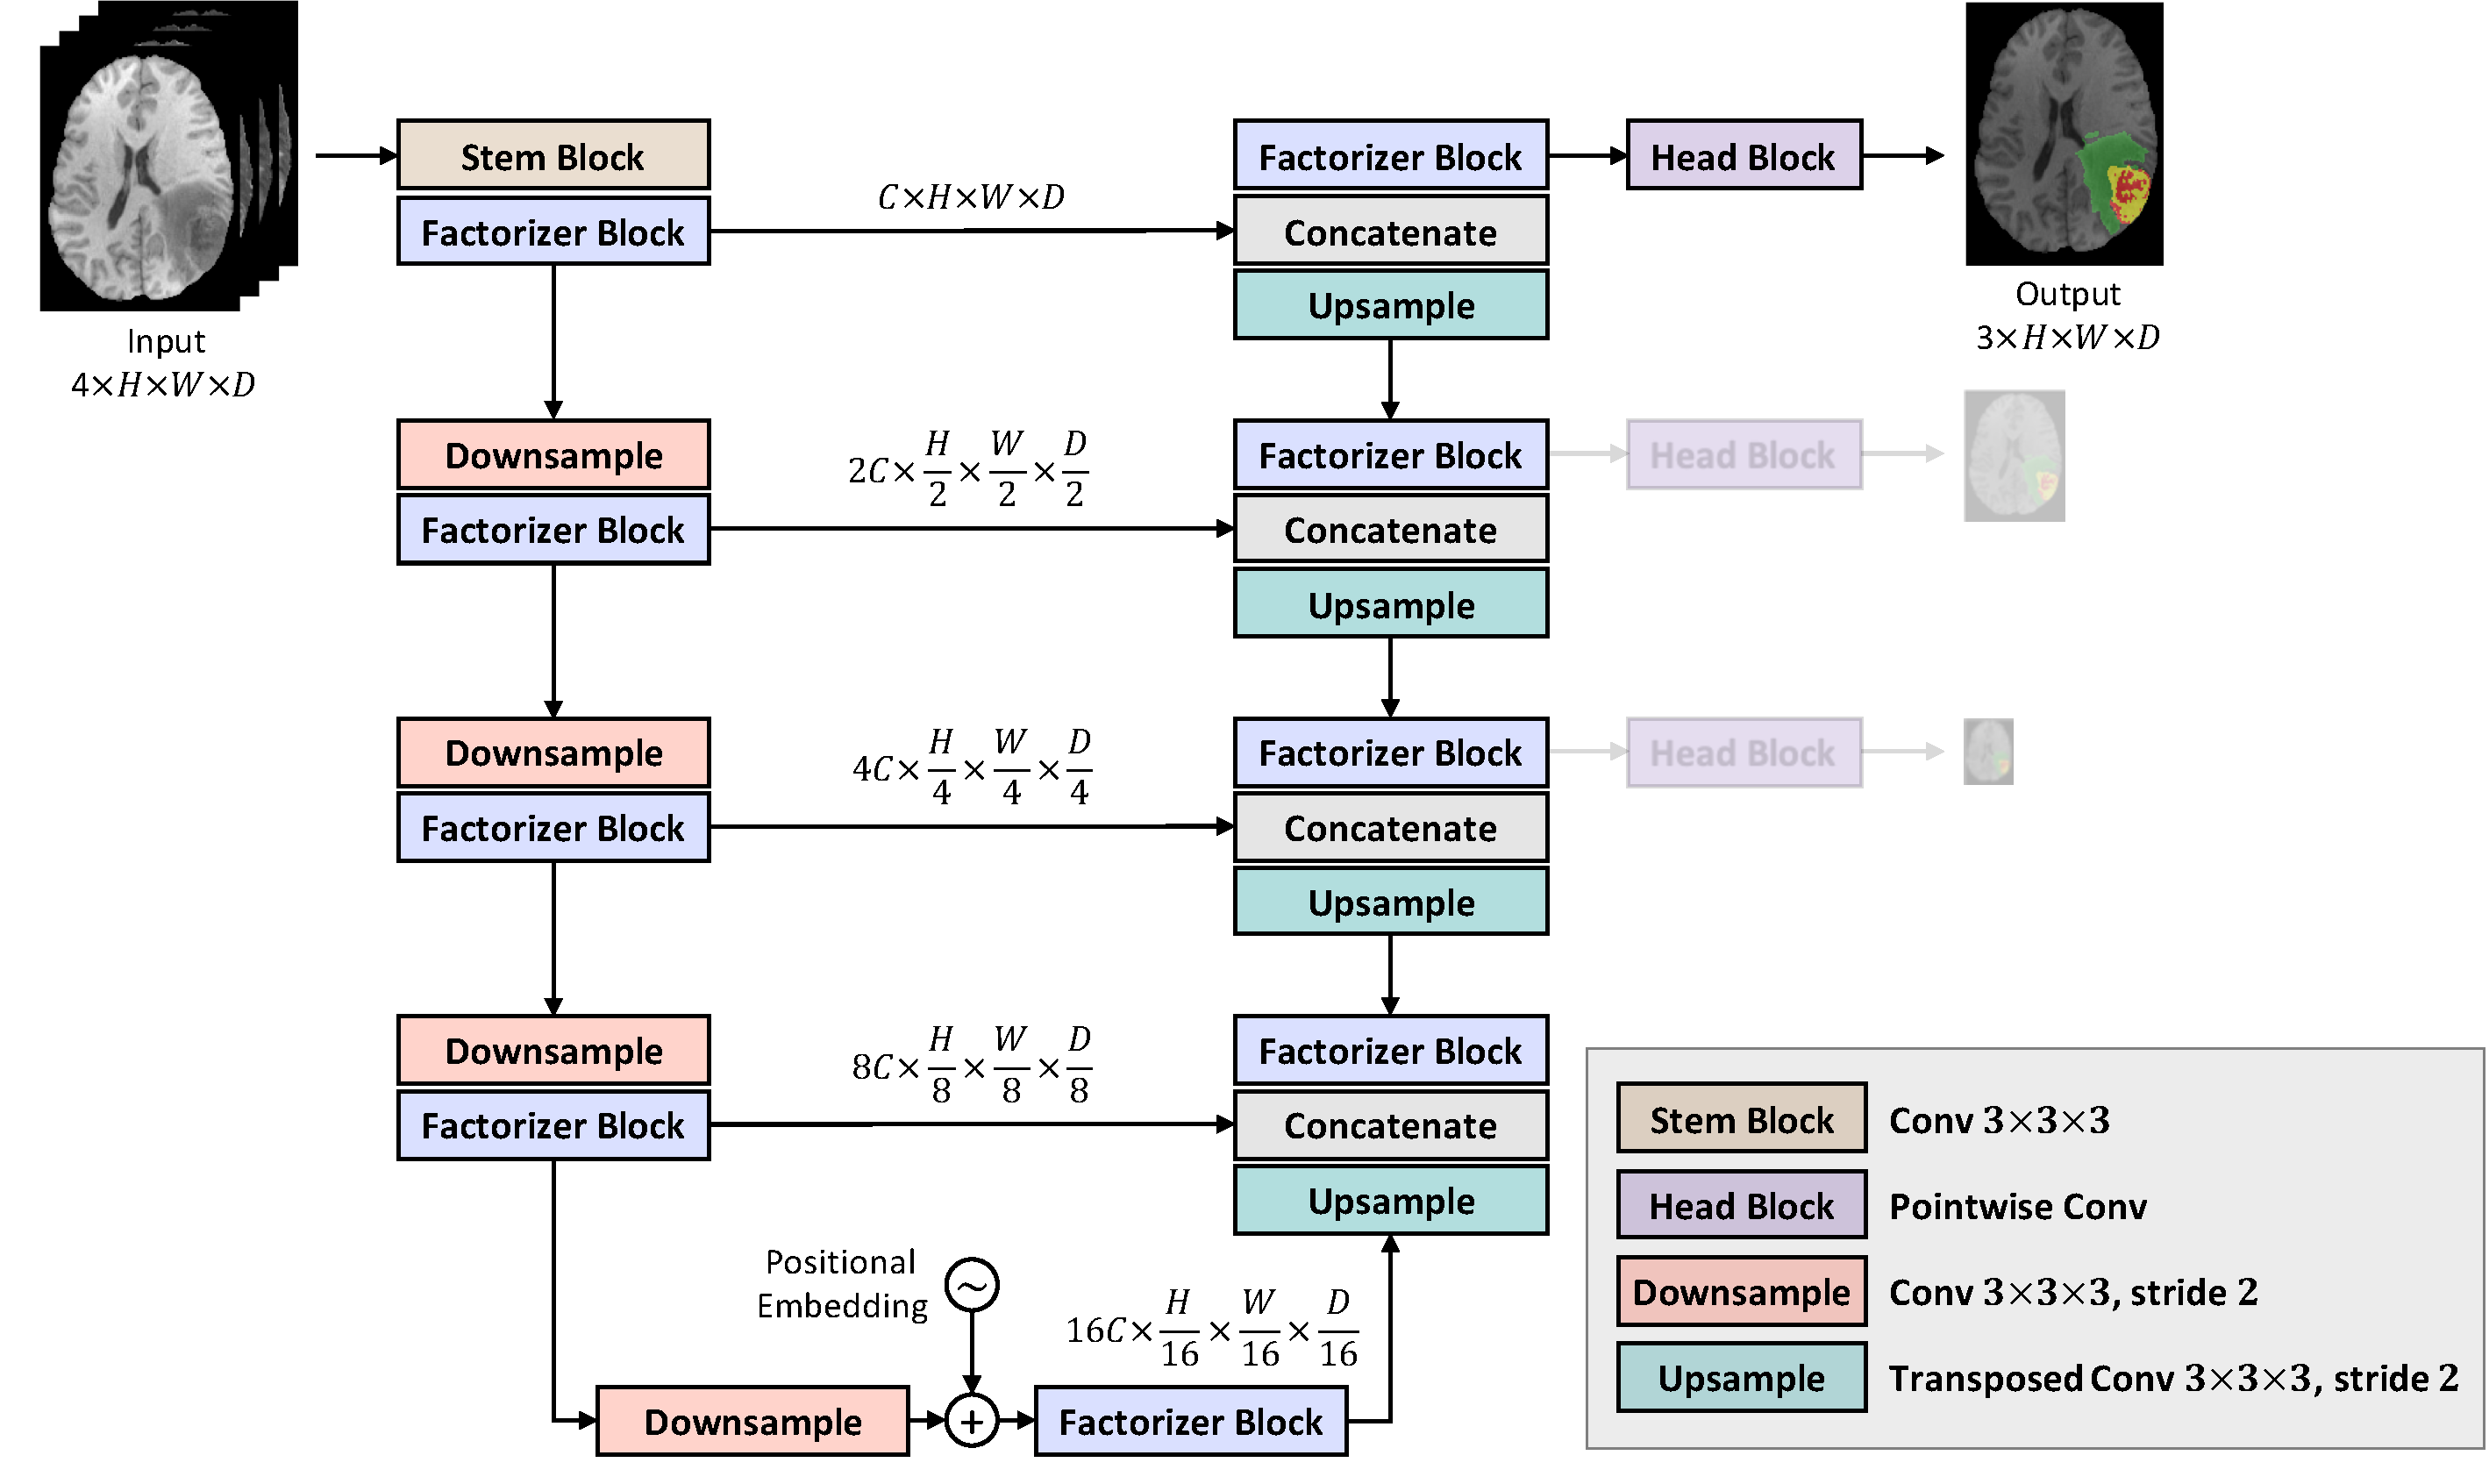
\includegraphics[width=.9\linewidth]{figures/factorizer.pdf}	
		\caption{The overall architecture of Factorizer.}
		\label{fig: factorizer}
	\end{figure}
	
	\subsection{Factorizer Block} \label{sec: factorizer block}
	
	A Factorizer block is constructed by replacing multi-head self-attention (MSA) module in a ViT block by a Wrapped NMF module (described in Section \ref{sec: wrapped nmf}). As shown in Figure \ref{fig: factorizer block}, a Factorizer block comprises NMF module and MLP, each of which follows a LayerNorm and is followed by a residual connection, that is,
	\begin{align}
		\label{eq: factorizer block}
		& \bm{\mathcal{Z}}'= \text{WrappedNMF}(\text{LayerNorm}(\bm{\mathcal{X}}) + \bm{\mathcal{X}}, \nonumber \\
		& \bm{\mathcal{Z}} = \text{MLP}(\text{LayerNorm}(\bm{\mathcal{Z}}')) + \bm{\mathcal{Z}}',
	\end{align}
	where MLP has two linear layers with GELU nonlinearity in between:
	\begin{equation}
		\label{eq: MLP}
		\text{MLP}(\bm{\mathcal{Z}}) = \text{PointwiseConv}(\text{GELU}(\text{PointwiseConv}(\bm{\mathcal{X}})).
	\end{equation}
	The number of input and output channels are the same, but the number of inner channels is set twice that of the input channels.
	
	\begin{figure}[!t]
		\centering
		\begin{subfigure}{.16\textwidth}
			\centering
			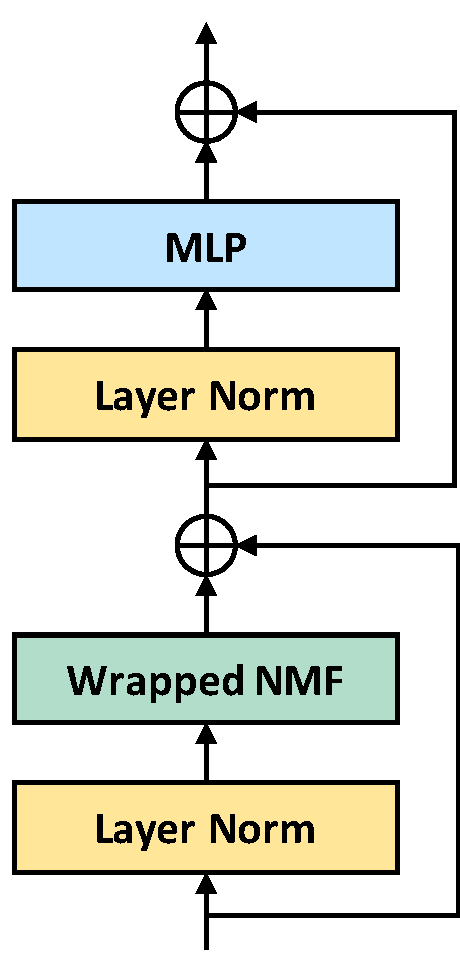
\includegraphics[width=.85\textwidth]{figures/factorizer_block.pdf}
			\caption{}
			\label{fig: factorizer block}
		\end{subfigure}
		\begin{subfigure}{.15\textwidth}
			\centering
			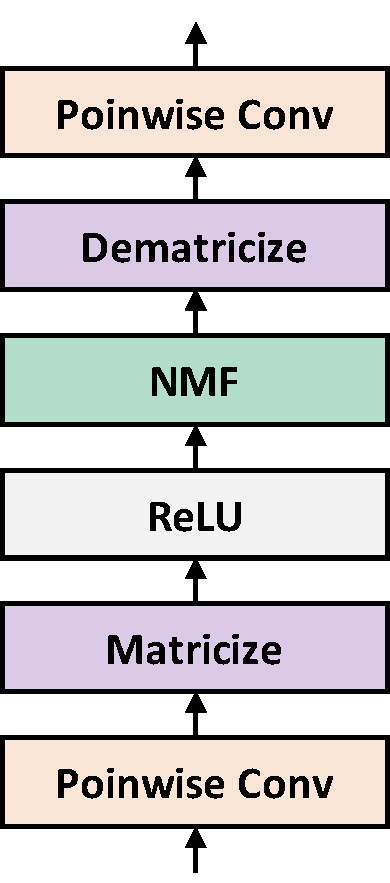
\includegraphics[width=.85\textwidth]{figures/wrapped_nmf.pdf}
			\caption{}
			\label{fig: wrapped nmf}
		\end{subfigure}
		\begin{subfigure}{.67\textwidth}
			\centering
			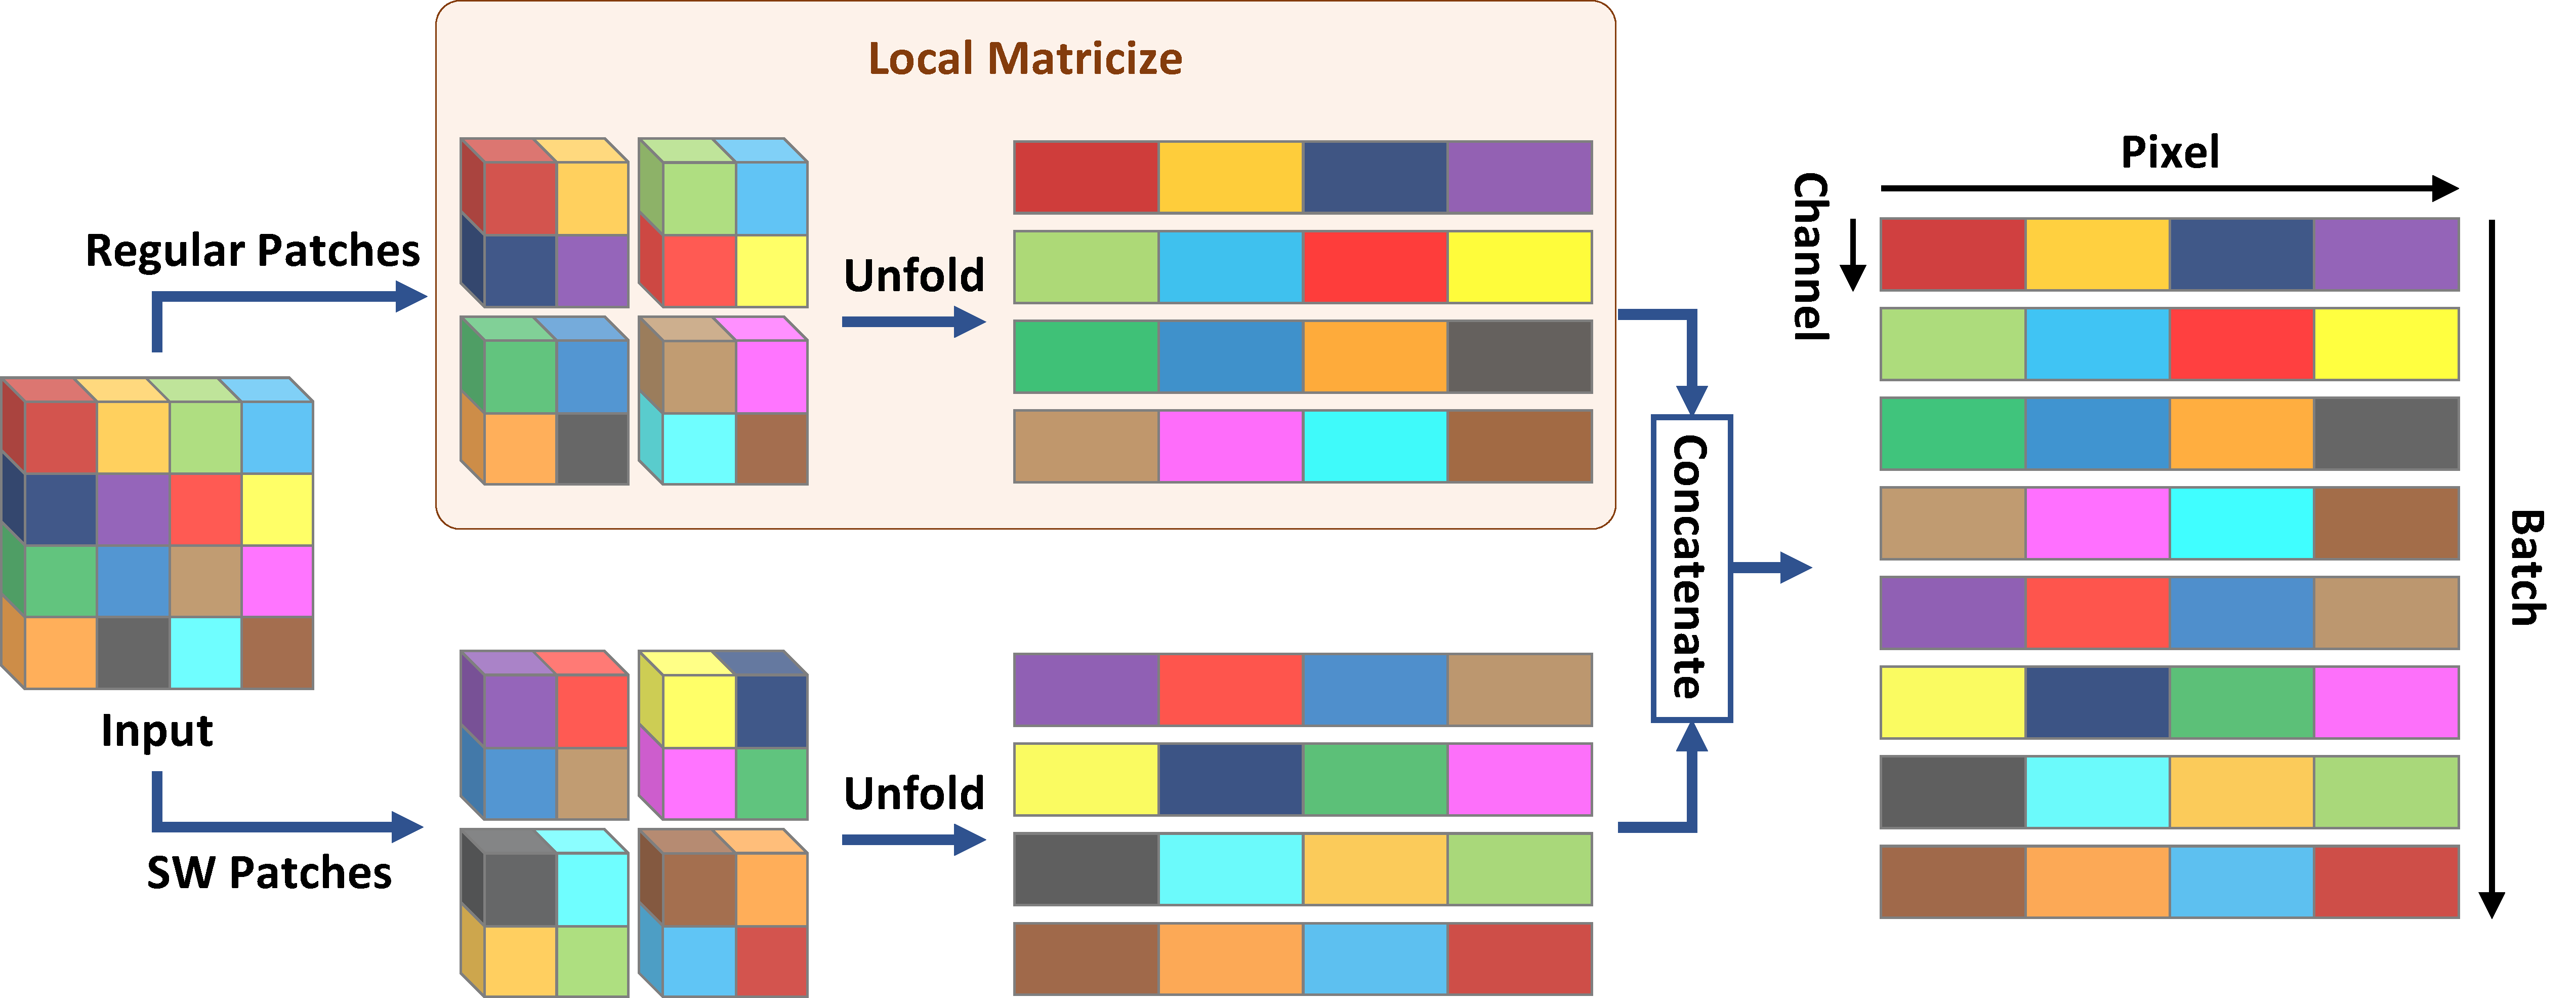
\includegraphics[width=.97\textwidth]{figures/sw-matricize.pdf}
			\caption{}
			\label{fig: sw-matricize}
		\end{subfigure}
		\caption{An overview of the Factorizer block and its components. (a) overall Factorizer block (b) Wrapped NMF module (c) An illustration of Swin Matricize on a 2D toy example.}
		\label{fig: factorizer block and its components}
	\end{figure}
	
	
	\subsection{Wrapped NMF Module} \label{sec: wrapped nmf}
	
	The integral component of Factorizer is the Wrapped NMF module, which relies on matricization (i.e., an operation that turns a tensor into a matrix) and nonnegative matrix factorization (NMF). As shown in \ref{fig: wrapped nmf}, a Wrapped NMF subblock first applies a pointwise convolution to linearly project each voxel. The output is then reshaped into a batch of matrices using a \textit{Matricize} operation, which is detailed later on in Section \ref{sec: matricize}. The resulting matrices pass through ReLU to clamp all their elements into nonnegative values and then low-rank approximated using NMF. The constructed matrices are reshaped back to their original size using the \textit{Dematricize} operation, i.e., the inverse of Matricize. Finally, another pointwise convolution is applied, yielding the output. More formally, Wrapped NMF can be computed as follows:
	\begin{align}
		\label{eq: wrapped nmf}
		& \bm{\mathcal{X}}^1 = \text{PointwiseConv}(\bm{\mathcal{X}}), \nonumber \\
		& \bm{\mathcal{X}}^2 = \text{Matricize}(\bm{\mathcal{X}}^1), \nonumber \\
		& \bm{\mathcal{X}}^3 = \text{NMF}(\text{ReLU}(\bm{\mathcal{X}}^2)), \nonumber \\
		& \bm{\mathcal{X}}^4 = \text{Dematricize}(\bm{\mathcal{X}}^3), \nonumber \\
		& \text{WrappedNMF}(\bm{\mathcal{X}}) = \text{PointwiseConv}(\bm{\mathcal{X}}^4),
	\end{align}
	where intermediate tensors $ \bm{\mathcal{X}}^i $s and the output have the same size as that of input $ \bm{\mathcal{X}} $.   
	
	
	\subsubsection{Matricize} \label{sec: matricize}
	
	Before applying any matrix factorization method, an input batch of multi-dimensional images, denoted by $ \bm{\mathcal{X}} \in \mathbb{R}^{B \times C \times H \times W \times D} $, must be turned into a batch of matrices, say $ \mathbf{Z} \in \mathbb{R}^{B' \times M \times N} $. This operation is called \textit{Matricize}. In this work, we propose three Matricize operations: i) Global Matricize, ii) Local Matricize, and iii) Shifted Window (SW) Matricize. Depending on which operation is used, different variants for Factorizer are obtained: i) Global Factorizer, ii) Local Factorizer, and iii) \textbf{S}hifted \textbf{Win}dow (Swin) Factorizer. The Matricize operations are described in the following.
	
	\paragraph{Global Matricize}
	This operation simply flattens the spatial dimensions and also divides the channels into multiple groups (analogous to heads of Multi-Head Self-Attention). More specifically, Global Matricize reshapes a batch of $ C $-channel 3D images $ \bm{\mathcal{X}} \in \mathbb{R}^{B \times C \times H \times W \times D} $ into a batch of matrices denoted by a 3D tensor $ \mathbf{Z} \in \mathbb{R}^{B(C/E) \times E \times HWD} $, where $ E $ is called the head dimension, i.e., the number of channels per head (or matrix). This operation is obviously suitable for modeling global context and imposes no locality inductive bias.
	
	\paragraph{Local Matricize}
	Global Matricize lacks a notion of locality which is typically useful for images, especially in low-data regimes. Local Matricize is proposed to mitigate this shortcoming by splitting an input $ \bm{\mathcal{X}} \in \mathbb{R}^{B \times C \times H \times W \times D} $ into a grid of non-overlapping patches of size $ (E, P, P, P) $. These patches are flattened spatially and then concatenated along the batch dimension, yielding a batch of matrices presented by the tensor $ \mathbf{Z} \in \mathbb{R}^{BCHW/(EP^3) \times E \times P^3} $. The entire procedure can be summarized by Einstein notation:
	\begin{equation}
		\label{eq: local matricize}
		\mathbf{Z}[b g_c g_h g_w g_d, e, p_e p_w p_d] = \bm{\mathcal{X}}[b, g_c e, g_h p_h, g_w p_w, g_d p_d]
	\end{equation}
	where $ (g_c, g_h, g_w, g_d) $ and  $ (e, p_h, p_w, p_d) $ indices correspond to grid and patch dimensions, respectively. In PyTorch and TensorFlow, such Einstein operations can be simply implemented using \texttt{rearrange} function from \texttt{einops} library. Once NMF is applied to the resulting batch of matrices, the inverse operation of Local Matricize, called Local Dematricize, must be applied to transform them back to the initial shape. Local Dematricize can be easily obtained by composing the inverses of sub-operations in reverse order. In practice, Local Dematricize can also be formulated and implemented as an Einstein operation. A PyTorch-style pseudocode of Local (De)matricize module is provided in Algorithm \ref{alg: local-swin-matricize}.
	
	Note that while Local Matricize seems to reshape an image in a similar way to the input patchifier of ViT, it concatenates patches along batch dimension rather than channel dimension. In fact, Local Matricize can be used when modeling within-patch interactions is desirable, which is different from ViT-based approaches, where interactions between embedded patches are typically modeled. 
	
	%\begin{equation}
	%	\label{eq: local dematricize}
	%	\bm{\mathcal{X}}[b, g_c e, g_h p_h, g_w p_w, g_d p_d] = \mathbf{Z}[b g_c g_h g_w g_d, e, p_e p_w p_d]
	%\end{equation}
	%
	
	\paragraph{Shifted Window Matricize.}
	While Local Matricize introduces locality to a model, voxels close to the boundaries of partitioning windows are not represented effectively. Since patches are low-rank approximated independently later on in an NMF layer, two neighboring boundary voxels from two adjacent patches are very likely to end up having excessively different feature maps in the output of the factorizer block, which in turn eventually makes the prediction less accurate for such voxels. To mitigate this problem, we utilize a shifted window approach proposed by \citet{liu2021swin} and introduce a Shifted Window (SW) Matricize operation, making the output feature maps smoother around boundaries. 
	
	An illustration of SW Matricize is provided in Figure \ref{fig: sw-matricize}. Here, in addition to regular patches similar to those extracted by Local Matricize, shifted window (SW) patches are also included. Let's $ \bm{\mathcal{X}} \in \mathbb{R}^{B \times C \times H \times W \times D} $ be the input and $ (P, P, P) $ the patch size. To extract SW patches, the input must be first shifted by the offset of $ (P/2, P/2, P/2) $ along spatial dimensions such that voxels shifted beyond the boundaries of the images are re-introduced at the first position, yielding a tensor of the same size $ B \times C \times H \times W \times D $. We call this operation \textit{Roll} (which can be implemented using \texttt{roll} function in PyTorch and TensorFlow). The resulting rolled tensor is then reshaped by Local Matricize to get SW patches. Finally, both the batches of regular and SW patches are concatenated along the batch dimension. Formally, SW Matricize is computed as follows:
	\begin{align}
		\label{eq: sw-matricize}
		& \bm{\mathcal{X}}^1 = \text{LocalMatricize}_{P}(\bm{\mathcal{X}}), \nonumber \\
		& \bm{\mathcal{X}}^2 = \text{LocalMatricize}_{P}(\text{Roll}_{P/2}(\bm{\mathcal{X}})), \nonumber \\
		& \text{SWMatricize}(\bm{\mathcal{X}}) = \text{Concatenate}(\bm{\mathcal{X}}^1, \bm{\mathcal{X}}^2),
	\end{align}
	where $ \text{LocalMatricize}_{P} $ denotes Local Matricize with a patch size of $ (P, P, P) $, and $ \text{Roll}_{P/2} $ denotes Roll operator with a shift $ (P/2, P/2, P/2) $. To build SW Dematricize, we need to reconstruct the image from both regular and SW patches independently then compute their average to achieve a smoother and more accurate feature maps. 
	%That is,
	%\begin{align}
	%	\label{eq: sw-demmatricize}
	%	& \bm{\mathcal{X}}^1 = \text{LocalMatricize}_{P}(\bm{\mathcal{X}}) \nonumber \\
	%	& \bm{\mathcal{X}}^2 = \text{LocalMatricize}_{P}(\text{Roll}_{P/2}(\bm{\mathcal{X}})) \nonumber \\
	%	& \text{SWMatricize}(\bm{\mathcal{X}}) = \text{Concatenate}(\bm{\mathcal{X}}^1, \bm{\mathcal{X}}^2)
	%\end{align}
	Further details are provided in Appendix \ref{app: matricize implementation details}, which includes a PyTorch implementation of SW (De)matricize module presented in Algorithm \ref{alg: local-swin-matricize}.
	
	\subsubsection{Nonnegative Matrix Factorization} \label{sec: nmf}
	
	Once the input is somehow transformed to a batch of matrices, and its negative elements are clipped to zero by ReLU, it is ready to be low-rank approximated by Nonnegative Matrix Factorization (NMF). This is the main component of a factorizer model that contributes most to modeling local or global context in an image.  
	
	NMF \citep{lee1999learning} seeks to approximate some given nonnegative matrix $ \mathbf{X} \in \mathbb{R}_{\ge 0}^{M \times N} $ by 
	\begin{equation}
		\label{eq: nmf}
		\mathbf{X} \approx \mathbf{F} \mathbf{G}^T,
	\end{equation}
	where $ \mathbf{F} \in \mathbb{R}_{\ge 0}^{M \times R} $ and $ \mathbf{G} \in \mathbb{R}_{\ge 0}^{N \times R} $ are factors, and the positive integer $ R \leq \min(M, N) $ is the rank. Once the factors $ \mathbf{F} $ and $ \mathbf{G}^T $ are somehow approximated, the NMF layer in a Factorizer block outputs the reconstructed matrix $ \hat{\mathbf{X}} = \mathbf{F} \mathbf{G}^T $. Various loss functions have been used to form the objective function and measure the quality of an approximation. Depending on the loss function, constraints, and regularization, many variants of NMF have been proposed. In this work, we use a standard NMF with the squared error, which is the most-widely used variant for images, to find factors by solving
	\begin{equation}
		\label{eq: nmf objective}
		\underset{\mathbf{F} \geq 0, \mathbf{G} \geq 0}{\text{minimize}} \ \lVert \mathbf{X} - \mathbf{F} \mathbf{G}^T \rVert^2.
	\end{equation}
	In general, problem \eqref{eq: nmf objective} is nonconvex, and finding global minima is NP-hard. However, numerous iterative algorithms have been proposed to find a ``good local minimum". The  majority of existing methods are based on a block coordinate descent (BCD) scheme (a.k.a alternating optimization), where the objective function is iteratively minimized with respect to one factor while the other factor is kept fixed. That is, the convex subproblems
	\begin{align}
		\label{eq: nmf bcd subproblems} 
		\mathbf{F} \gets \underset{\mathbf{F} \geq 0}{\argmin} \ \lVert \mathbf{X} - \mathbf{F} \mathbf{G}^T  \rVert^2, \qquad & 
		\mathbf{G} \gets \underset{\mathbf{G} \geq 0}{\argmin} \ \lVert \mathbf{X}^T - \mathbf{G} \mathbf{F}^T \rVert^2,
	\end{align}
	are exactly or approximately solved alternately.This ensures that the objective function value does not increase after each update and guarantees convergence to a stationary point under some mild conditions \citep{grippo2000convergence}. 
	
	\begin{algorithm}[!t]	
		\caption{Multiplicative update solver for NMF ($ \circ $ denotes element-wise matrix product). \label{alg: multiplicative update}}
		\DontPrintSemicolon
		\KwIn{$ \mathbf{X} \in \mathbb{R}_{\ge 0}^{M \times N} $ (input matrix), $ R $ (rank); $ T $ (\# iterations)}
		\KwOut{$ \mathbf{\hat{X}} \in \mathbb{R}_{\ge 0}^{M \times N} $ (low-rank approximated matrix)}
		Initialize factors $ \mathbf{F} \in \mathbb{R}_{\ge 0}^{M \times R} $ and $ \mathbf{G} \in \mathbb{R}_{\ge 0}^{N \times R} $\;
		\For{$ t = 1, \dots, T $}{
			\vspace{5pt}		
			$ \displaystyle \mathbf{F} \gets \mathbf{F} \circ \frac{\mathbf{X} \mathbf{G}}{\mathbf{F} \mathbf{G}^T \mathbf{G}} $\;
			\vspace{5pt}
			$ \displaystyle \mathbf{G} \gets \mathbf{G} \circ \frac{\mathbf{X}^T \mathbf{F}}{\mathbf{G} \mathbf{F}^T \mathbf{F}} $\;
			\vspace{5pt}		
		}
		\Return $ \displaystyle \mathbf{\hat{X}} = \mathbf{F} \mathbf{G}^T $
	\end{algorithm}
	
	\begin{algorithm}[!t]	
		\caption{Hierarchical alternating least squares for NMF. \label{alg: hals}}
		\DontPrintSemicolon
		\KwIn{$ \mathbf{X} \in \mathbb{R}_{\ge 0}^{M \times N} $ (input matrix), $ R $ (rank); $ T $ (\# iterations)}
		\KwOut{$ \mathbf{\hat{X}} \in \mathbb{R}_{\ge 0}^{M \times N} $ (low-rank approximated matrix)}
		Initialize factors $ \mathbf{F} \in \mathbb{R}_{\ge 0}^{M \times R} $ and $ \mathbf{G} \in \mathbb{R}_{\ge 0}^{N \times R} $\;
		\For{$ t = 1, \dots, T $}{
			$ \mathbf{A} =  \mathbf{X} \mathbf{G} $, $ \mathbf{B} = \mathbf{G}^T \mathbf{G} $\;
			%		\tcp{Update $ \mathbf{F} $}
			\For{$ r = 1, \dots, R $}{				
				$ \displaystyle \mathbf{F}[:,r] \gets \max(0, \frac{\mathbf{A}[:,r] - \sum_{\ell \neq r} \mathbf{B}[\ell,r] \mathbf{F}[:,\ell]}{\lVert \mathbf{G}[:,r] \rVert^2}) $
			}
			$ \mathbf{A} =  \mathbf{X}^T \mathbf{F} $, $ \mathbf{B} = \mathbf{F}^T \mathbf{F} $\;
			%		\tcp{Update $ \mathbf{G} $}
			\For{$ r = 1, \dots, R $}{					
				$ \displaystyle \mathbf{g}[:,r] \gets \max(0, \frac{\mathbf{A}[:,r] - \sum_{\ell \neq r} \mathbf{B}[\ell,r] \mathbf{G}[:,\ell]}{\lVert \mathbf{F}[:,r] \rVert^2}) $
			}
			%		$ \displaystyle \mathbf{F} \gets [\mathbf{f}_1 | \dots | \mathbf{f}_R] $, $ \mathbf{G} \gets [\mathbf{g}_1 | \dots | \mathbf{g}_R] $\;		
		}
		\Return $ \displaystyle \mathbf{\hat{X}} = \mathbf{F} \mathbf{G}^T $
	\end{algorithm}
	
	Among numerous BCD-based algorithms for NMF, Multiplicative Update (MU) \citep{lee1999learning} is the best-known due to the advantage of being easy-to-implement and scalable. MU enforces nonnegativity constraint by updating the previous values of a factor matrix by multiplication with a nonnegative scale factor. A pseudocode of MU is pretended in Algorithm \ref{alg: multiplicative update}. However, slow convergence of MU has been pointed \citep{gillis2020nonnegative}, and hence more effective algorithms, such as Hierarchical Alternating Least Squares (HALS) \citep{cichocki2009fast}, with faster convergence have been introduced. HALS updates a factor matrix, say $ \mathbf{F} = [\mathbf{f}_1 | \dots | \mathbf{f}_R] $, with inner iterations, in which the columns $ \mathbf{f}_r $s are updated by solving the following subproblem
	\begin{equation}
		\label{eq: hals subproblem} 
		\mathbf{f}_r \gets \underset{\mathbf{f}_r \geq 0}{\argmin} \ \lVert \mathbf{E}_r - \mathbf{f}_r \mathbf{g}_r^T \rVert^2,
	\end{equation}
	where $ \mathbf{E}_r = \mathbf{X} - \sum_{\ell \neq r}^{R} \mathbf{f}_\ell \mathbf{g}_\ell^T $ is the residual matrix, which is, in fact, approximated by a rank-one matrix. An encouraging aspect of HALS is that each subproblem \eqref{eq: hals subproblem} can be easily shown to have a closed-form solution:
	\begin{equation}
		\label{eq: hals subproblem solution} 
		\mathbf{f}_r^* \gets \max(0, \frac{\mathbf{E}_r \mathbf{g}_r}{\lVert \mathbf{g}_r \rVert^2}).
	\end{equation}
	Similarly, the update formula for columns of $ \mathbf{G} $ can be derived. Note that HALS is a $ 2R $-block coordinate descent procedure, where at each outermost iteration, first the columns of $ \mathbf{F} $ and then the columns of $ \mathbf{G} $ are updated. Algorithm \ref{alg: hals} provides pseudocode of HALS (further details on MU and HALS can be found in \citep{gillis2020nonnegative}, Chapter 8). 
	
	A special case of NMF is $ R = 1 $; i.e., $ \mathbf{X} \approx \mathbf{f} \mathbf{g}^T $, where $ \mathbf{f} \in \mathbb{R}_{\ge 0}^M $ and $ \mathbf{g} \in \mathbb{R}_{\ge 0}^N $; for which one can easily investigate that both MU and HALS are simplified to the same update rule:
	\begin{align}
		\label{eq: rank-one update formulas} 
		\mathbf{f} \gets \frac{\mathbf{X} \mathbf{g}}{\lVert \mathbf{g} \rVert^2}, \qquad &  \mathbf{g} \gets \frac{\mathbf{X} \mathbf{f}}{\lVert \mathbf{f} \rVert^2}.
	\end{align}
	In this paper, all Factorizer models are trained with $ R = 1 $, and compression ratios (and somewhat reconstruction errors) are controlled by adjusting the head dimension (i.e., the number of rows in a matrix, as discussed in \ref{sec: matricize}) to sufficiently small values. This means that a matricize operation transforms an image into a batch of such fat matrices (whose number of columns are far more than rows) that rank-one approximation would suffice in practice. This greatly simplifies a factorizer model and improves the interpretability while yielding better performance in segmentation. However, in one of our ablation studies (see Section \ref{sec: ablation studies}), we experimented with both MU and HALS for $ R > 1 $ to investigate the impact of rank in the inference phase.
	
	It is worth mentioning that not all NMF algorithms and their settings can be used in the NMF layer of a Factorizer block. The utilized algorithm must have some properties so that we can ultimately train the Factorizer model successfully in an end-to-end fashion using a gradient descent-based optimizer on GPU(s) in an existing deep learning framework, such as PyTorch. Firstly, the algorithm should be backpropagation-friendly and amenable to automatic differentiation, that is $ \frac{\partial \hat{\mathbf{X}}}{\partial \mathbf{X}} $ should not only be well-defined and somewhat smooth but also computable by an existing deep learning framework, such as PyTorch, so that we can practically train the Factorizer model in an end-to-end fashion using a gradient descent optimizer. Another related aspect is that the gradient $ \frac{\partial \hat{\mathbf{X}}}{\partial \mathbf{X}} $, as explained in \citep{geng2021attention}, stats to vanish during backpropagation after some iterations. Therefore, the number of outer iterations $ T $ in an NMF algorithm should be limited in order to have stable gradients. For MU and HALS, $ T = 5 $ is a reasonable choice in practice. Finally, update rules should be also friendly to GPU parallel processing for exploiting GPUs to train Factorizers in a reasonable amount of time. Taking all these factors into account, MU and HALS are appropriate choices. While HALS has better convergence properties, MU is more favorable for GPU training due to unparallelizable inner iterations of HALS.
	
	
	\section{Experiments} \label{sec: experiments}
	
	
	\subsection{dataset.} 
	
	We evaluate the effectiveness of our models in segmenting brain tumors on the Brain Tumour Segmentation (BraTS) dataset \citep{brats1, brats2, brats3} from Medical Segmentation Decathlon (MSD) (Task 1) \citep{antonelli2021medical}. The BraTS training set consists of 484 multiparametric MRI (mpMRI) scans from patients diagnosed with either low-grade glioma or high-grade glioma (glioblastoma). Each scan comes with four 3D MRI sequences, namely T2 Fluid-Attenuated Inversion Recovery (FLAIR), native T1-weighted (T1), post-Gadolinium contrast T1-weighted (T1gd), and T2-weighted (T2). Once images are prepossessed; i.e., rigidly co-registered the same anatomical template, resampled to the same voxel spacing $ 1 \text{mm}^3 $, and skull-stripped; the ground truths are manually created by experts who label each voxel as enhancing tumor (ET), edema (ED), necrotic and non-enhancing tumor (NCR/NET), or everything else. However, for evaluation, the 3 nested subregions, namely enhancing tumor (ET), tumor core (TC--i.e., the union of ED and NCR/NET), and whole tumor (WT) are used (see the sample ground truths in Figure \ref{fig: sample results})
	
	
	\subsection{Setup} \label{sec: setup}
	
	All the models were implemented using PyTorch \citep{PyTorch2019} and MONAI \citep{monai2021} frameworks and trained on NVIDIA P100 GPUs. We followed the same training workflow in all the experiments. In the following, we first provide the details of this workflow and baseline models, then present the evaluation protocol and the results.
	
	\paragraph{Preprocessing.} 
	For each scan in the BraTS dataset, a 4-channel 3D image as the input was first constructed by concatenating the four modalities, FLAIR, T1, T1gd, and T2. The image and its ground truth were then cropped with a minimal box filtering out zero regions. The image was normalized channel-wise using z-score to have intensities with zero mean and unit variance. Random patches of size $ (128, 128, 128) $ were extracted from the images for training. To reduce overfitting, we used data augmentation techniques, including random affine transform, random flip along each spatial dimension, additive Gaussian noise, random Gaussian smoothing, random scale intensity,  random shift intensity, and random gamma transform. The further details are provided in Appendix \ref{app: data augmentation pipeline}.
	
	\paragraph{Training.} 
	All models were trained for 100k steps with batch size 2 (one sample per GPU) using AdamW optimizer with a base learning rate of $ 1\mathrm{e}{-4} $, weight decay of $ 1\mathrm{e}{-2} $, warmup of 2k steps, and cosine annealing scheduler. The loss function is a combination of \textit{soft Dice loss} \citep{milletari2016v} and cross-entropy loss, defined as
	\begin{equation}
		\label{eq: loss}
		\mathcal{L}(\mathbf{G}, \mathbf{Y}) = \mathcal{L}_{\text{Dice}}(\mathbf{G}, \mathbf{Y}) + \mathcal{L}_{\text{CE}}(\mathbf{G}, \mathbf{Y}),
	\end{equation}
	where
	\begin{align}
		\label{eq: dice and cross-entropy loss}
		\mathcal{L}_{\text{Dice}}(\mathbf{G}, \mathbf{P}) = 1 - \frac{2 \langle \mathbf{G}, \mathbf{Y} \rangle}{\lVert\mathbf{G}\rVert^2 + \lVert\mathbf{Y}\rVert^2}, \qquad & \mathcal{L}_{\text{CE}}(\mathbf{G}, \mathbf{Y}) =  -\frac{1}{N}\langle \mathbf{G}, \log(\mathbf{Y}) \rangle,
	\end{align}
	where $ \mathbf{G} \in \{0, 1\}^{J \times N} $ and $ \mathbf{Y} \in [0, 1]^{J \times N} $ represent the one-hot encoded ground truth and the predicted probability map for each voxel, respectively, with $ J $ denoting the number of segmentation classes and $ N $ denoting the number of voxels in the patch. The three deep supervision outputs and the corresponding downsampled ground truths are used for computing the final loss. The training objective is the weighted mean of the losses at all these resolutions, with the weights being 1, 0.5, and 0.25 at resolutions $ 128^3 $, $ 64^3 $, and $ 32^3 $, respectively.
	
	\paragraph{Inference.} 
	A test image in the inference was first subjected to z-score intensity normalization, then the prediction was made using a sliding window approach with a 50\% overlap and a window size of $ 128 \times 128 \times 128 $ (same as the patch size used in training). Finally, the resulting probabilities were thresholded by 0.5 to obtain a binary segmentation map.
	
	\paragraph{Evaluation Metrics.}
	The Dice score and Hausdorff Distance 95\% (HD95) were used as metrics to asses the performance of models in our experiments. For each segmentation region, Dice score measures the voxel-wise overlap between the ground truth and the prediction, defined as
	\begin{equation}
		\label{eq: dice metric}
		\text{Dice}(\mathbf{g}, \mathbf{p}) = \frac{2 \sum_{n=1}^{N} g_n p_n}{\sum_{n=1}^{N} g_n + \sum_{n=1}^{N}, p_n}
	\end{equation}	
	where $ g_n \in \{0, 1\} $ and $ p_n \in \{0, 1\} $ represent the ground truth and the binary prediction for a voxel, respectively, and $ N $ is the number of voxels. If both the ground truth and the prediction do not have any nonzero values, that is the denominator of equation \eqref{eq: dice metric} is zero, the Dice score is defined as 1. Hausdorff Distance (HD) evaluates the distance between the boundaries of ground truth and prediction. HD is defined as follows:
	\begin{equation}
		\label{eq: hd metric}
		\text{HD}(G, P) = \max\{ \underset{\mathbf{g} \in G}{\max}\ \underset{\mathbf{p} \in P}{\min}\ \lVert \mathbf{g} - \mathbf{p} \rVert, \underset{\mathbf{p} \in P}{\max}\ \underset{\mathbf{g} \in G}{\min}\  \lVert \mathbf{p} - \mathbf{g} \rVert \},
	\end{equation}
	where $ G $ and $ P $ denote the set of all voxels on the surface of ground truth and prediction, respectively. HD95 is a more robust version to outliers, which calculates the 95\% quantile rather than the maximum of surface distances.
	
	\paragraph{Models.} 
	In all the experiments, the number of output channels of the stem block was 32. The patch size of Local and SW Matricize was set to $ (8, 8, 8, 8) $. In NMF modules, the factor matrices were initialized with uniform distribution $ \mathcal{U}(0, 1) $. In training, we used a rank-one approximation ($ R = 1 $) with $ T = 5 $ outer iterations of HALS (which is equivalent to MU for $ R = 1 $), as described in Section \ref{sec: nmf}. 
	
	To make a fair comparison between factorizer and baseline models, we neutralize the effect of architectural variability by keeping the overall architecture of baselines the same as that of Factorizer and only changing encoder and decoder blocks. This helps to better investigate the impact of blocks rather than architectures. Three models are used as baselines, all of which follow the same overall architecture illustrated in Figure \ref{fig: factorizer}, except that each has a different encoder and decoder block. The baselines are detailed in the following: 
	\begin{itemize}
		\item U-Net: This model is based on 3D U-Net \citep{cciccek20163d} with minor modifications. Each encoder (and decoder) block is composed of two convolutions with a kernel size of $ (3, 3, 3) $. Each convolutional layer is followed by LeakyReLU nonlinearity and Group Normalization (with a group size of 8) in order. This model does not have any positional embedding in its bridge since CNNs already have some notion of position. This model is very similar to nnU-Net \citep{isensee2018no}
		
		\item Res-U-Net: ResNet block \citep{he2016deep} is the cornerstone of Res-U-Net. This block is similar to that of U-Net, except that it has residual connection after the last Group Normalization. This model is very similar to SegResNet \citep{myronenko20183d}.
		
		\item Performer: The encoder and decoder blocks of this model are based on ViT (note that the input is first flattened into a sequence of voxels before feeding to a ViT block). However, attention scales quadratically with the number of voxels, hence is prohibitively expensive in our case, where the input can have up to $ 128^3 $ voxels. Therefore, we replace original attention layers of a ViT block with FAVOR+ (Fast Attention Via positive Orthogonal Random features) used in Performer, recently proposed by \citet{choromanski2020rethinking} as a linearly scalable alternative to Transformer. FAVOR+ gives an unbiased estimate of attention using only linear (as opposed to quadratic) time and space complexity. Note that except for the attention layers, the rest of the components of this baseline are the same as those of Factorizer.
		
		
	\end{itemize}
	
	
	\subsection{Results}
	
	\begin{table}[!t]
		\caption{Comparison of different models on the BraTS dataset. Scores are obtained by 5-Fold cross-validation. The asterisks indicate how significantly our models scores differ from those of baselines according to pairwise Wilcoxon signed-rank test (*: $\text{p-value} < 0.05 $; **: $ \text{p-value} < 0.01 $; ***: $ \text{p-value} < 0.001 $; and ****: $ \text{p-value} < 0.0001 $).}
		\label{tab: validation results}
		\newcolumntype{P}[1]{>{\centering\arraybackslash}p{#1}}
		\def\arraystretch{1.3}
		\resizebox{\textwidth}{!}{	
			\begin{tabular}{m{.2\textwidth} | P{.1\textwidth} P{.1\textwidth} | *{4}{P{.08\textwidth}} | *{4}{P{.08\textwidth}}}		
				\toprule
				
				\multirow{2}{*}{Model} & \multirow{2}{*}{\#Params} & \multirow{2}{*}{FLOPs} & \multicolumn{4}{c|}{Dice (\%)}                                                                     & \multicolumn{4}{c}{Hausdorff 95\% (mm)}  \\ \cline{4-11} 	
				&                           &                        & ET                   & TC                   & WT 				  & \multicolumn{1}{|c|}{Avg.} & ET & TC & WT & \multicolumn{1}{|c}{Avg.} \\ 
				
				\hline
				
				U-Net                  & 28.7M                     & 1264.7G                & 75.89 &    81.94 &    90.09 & \multicolumn{1}{|c|}{82.64}     &  8.61 &   9.13 &   9.31  &  \multicolumn{1}{|c}{9.19}    \\
				Res-U-Net              & 28.9M                     & 1280.8G                &         77.95 &    82.49 &    \textbf{90.39}$ ^{*} $  & \multicolumn{1}{|c|}{83.61}     &   6.08 &   8.18 &   \textbf{8.06}$ ^{**} $    &  \multicolumn{1}{|c}{7.52} \\
				Performer              & 6.7M                      & 321.8G                 &   78.43                   &       82.34               &   88.72  & \multicolumn{1}{|c|}{83.16}     &  6.72  & 9.78  & 12.93   &  \multicolumn{1}{|c}{10.21}     \\ 
				
				\hline
				
				Global Factorizer      & 5.9M                      & 282.2G                 &         78.20 &    82.86 &    88.65    & \multicolumn{1}{|c|}{83.24}     &   6.67 &   9.53 &  11.69  &  \multicolumn{1}{|c}{9.71}      \\
				Local Factorizer       & 5.9M                      & 283.9G                 &          78.67 &    82.85 &    89.30    & \multicolumn{1}{|c|}{83.61}     &  5.29 &   7.77 &   8.91  &  \multicolumn{1}{|c}{7.41}      \\
				Swin Factorizer        & 5.9M                      & 290.4G                 &       \textbf{79.33} &    \textbf{83.14}$ ^{***} $ &    90.16    & \multicolumn{1}{|c|}{\textbf{84.21}$ ^{**} $}     &   \textbf{4.91}$ ^{**} $ &   \textbf{7.31}$ ^{*} $ &   8.23    &  \multicolumn{1}{|c}{\textbf{6.89}$ ^{*} $}      \\ 
				
				\bottomrule
			\end{tabular}
		}
	\end{table}
	
	\begin{figure}[!t]
		\centering
		\begin{subfigure}{.5\textwidth}
			\centering
			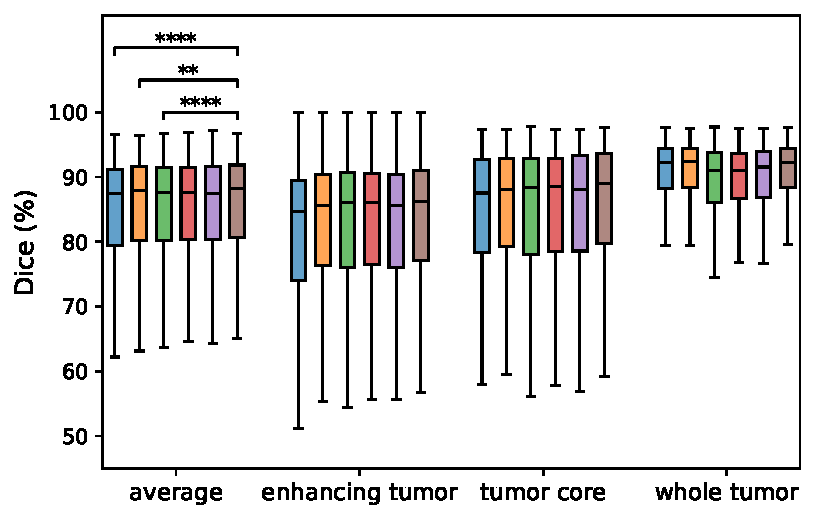
\includegraphics[width=.95\textwidth]{figures/dice_boxplot.pdf}
			\caption{}
		\end{subfigure}%
		\begin{subfigure}{.5\textwidth}
			\centering
			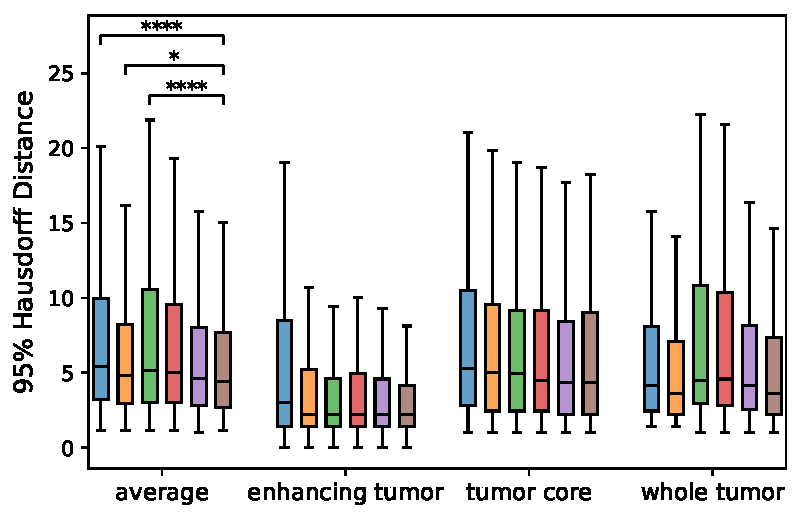
\includegraphics[width=.95\textwidth]{figures/hd_boxplot.pdf}
			\caption{}
		\end{subfigure}
		
		\begin{subfigure}{\textwidth}
			\centering
			
\includegraphics[width=.8\textwidth]{figures/legend.pdf}
			%		\caption{}
		\end{subfigure}
		\caption{The Dice score and 95\% Hausdorff distance of different models on the BraTS datasest. The asterisks indicate statistical significance according to pairwise Wilcoxon signed-rank test (*: $\text{p-value} < 0.05 $; **: $ \text{p-value} < 0.01 $; ***: $ \text{p-value} < 0.001 $; and ****: $ \text{p-value} < 0.0001 $).}
		\label{fig: scores boxplot}
	\end{figure}  
	
	\paragraph{Quantitative Evaluation.}
	For all the experiments, we performed 5-fold cross-validation to estimate how capable our models are in generalizing to unseen data. Pairwise Wilcoxon signed-rank test was also for comparing the performance of our models with that of the baselines. The results on the BraTS dataset are reported in Table \ref{tab: validation results} and illustrated by box plots in Figure \ref{fig: scores boxplot}.
	
	Swin Factorizer was superior to all the other models, which achieved an average Dice of 84.21\% and HD95 of 6.89, significantly outperforming Res-U-Net, the best baseline, with p-values of $ < 0.01 $ for average Dice and $ < 0.05 $ for average HD95, while requiring substantially fewer computations. Swin Factorizer was the best-performing on ET and TC subregions, particularly yielding a Dice of 83.14\% on TC, which is significantly higher than the others with $ \text{p-value} < 0.001 $. Local Factorizer was our second-best model, and its performance was comparable with that of Res-U-Net. More specifically, Local Factorizer outperformed Res-U-Net on ET and TC while underperforming on WT. As shown in Figure \ref{fig: dice_vs_flops}, while achieving competitive performance over U-Net and Res-U-Net, Factorizer models have much fewer parameters and are significantly cheaper, taking over four times lower theoretical computational cost (FLOPs).
	
	\begin{figure}[!t]
		\centering
		\begin{subfigure}{.5\textwidth}
			\centering
			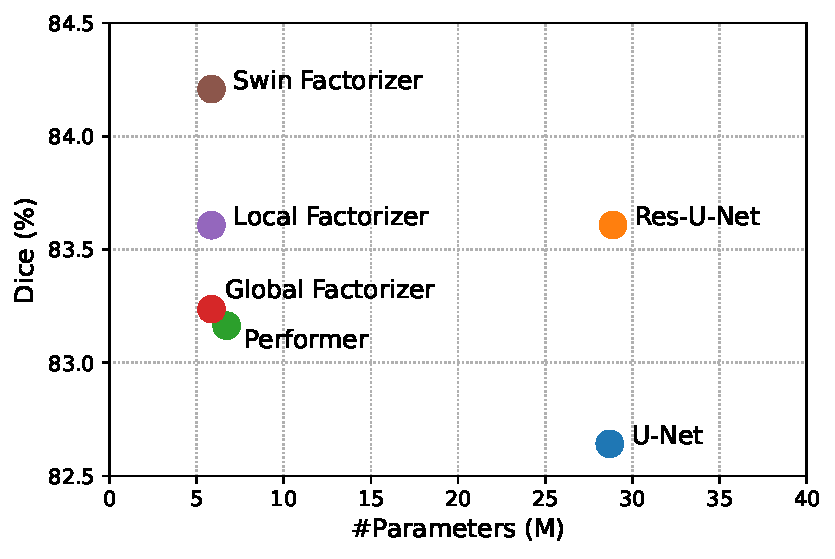
\includegraphics[width=.95\textwidth]{figures/dice_vs_params.pdf}
			\caption{}
		\end{subfigure}%
		\begin{subfigure}{.5\textwidth}
			\centering
			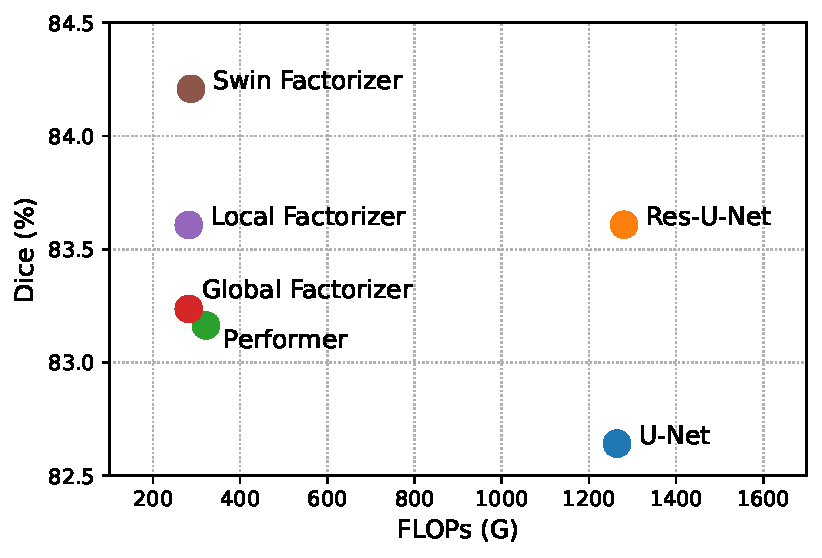
\includegraphics[width=.95\textwidth]{figures/dice_vs_flops.pdf}
			\caption{}
		\end{subfigure}
		\caption{Performance of Factorizer models in terms of average Dice on BraTS, versus their speed in terms of the number of FLOPs (left) and versus the number of parameters (right).}
		\label{fig: dice_vs_flops}
	\end{figure}
	
	Performer is the Transformer-based counterpart of Global Factorizer in the sense that they both only exploit global context without imposing any locality inductive bias in their blocks. However, while having lower computational complexity, Global Factorizer, with an average Dice score of 83.24\% and an average HD95 of 9.71, marginally outperformed Performer, with an average Dice score of 83.16\% and an average HD95 of 10.21. Local Factorizer improved the performance of Global Factorizer by exploiting locality, particularly with the average HD95 significantly dropping from 9.71 to 7.41 ($ \text{p-value} < 0.0001 $). As expected, Swin Factorizer improved all the scores of Local Factorizer, which is consistent with the fact that Swin Factorizer modifies Local Factorizer by better representing the boundary voxels in Local Matricize. 
	
	
	\paragraph{Qualitative Comparisons.}
	Qualitative comparisons of glioma segmentation models are presented in Figure \ref{fig: sample results}. Swin Factorizer demonstrates superior performance in segmenting TC and ET. This capability is evident in row 1 (row 2), where Swin Factorizer more successfully delineates TC compared to the other models, which do not as accurately distinguish edema (normal tissues) from tumor core. Particularly, the CNN-based models, i.e., U-Net and Res-U-Net, misclassify a significantly larger part of edema (normal tissues) as necrosis (enhancing tumor). Row 3 exemplifies a successful detection of TC by Swin Factorizer, while the other models miss a fairly large necrotic region.
	
	
	\begin{figure}[!t]
		\newcommand{\imagewithdice}[2]{
			\begin{tikzpicture}[every node/.style={inner sep=0, outer sep=0}]
				\node (image) at (0,0) {\includegraphics[width=1.0\textwidth]{#1}};
				\node[white, anchor=west] (dice) at (-1.15, -1.15) {\fontfamily{phv}\scriptsize\textbf{#2}};
			\end{tikzpicture}
			\vspace*{-15pt}	
		}
		\centering
		
		%	\begin{subfigure}{.167\textwidth}
		%		\centering
		%		\imagewithdice{figures/qualitative_results/gt_BraTS_078.pdf}{}
		%	\end{subfigure}%
		%	\begin{subfigure}{.167\textwidth}
		%		\centering
		%		\imagewithdice{figures/qualitative_results/swin-factorizer_pred_BraTS_078.pdf}{71.0}
		%	\end{subfigure}%
		%	\begin{subfigure}{.167\textwidth}
		%		\centering
		%		\imagewithdice{figures/qualitative_results/global-factorizer_pred_BraTS_078.pdf}{66.3}
		%	\end{subfigure}%
		%	\begin{subfigure}{.167\textwidth}
		%		\centering
		%		\imagewithdice{figures/qualitative_results/global-performer_pred_BraTS_078.pdf}{64.0}
		%	\end{subfigure}%
		%	\begin{subfigure}{.167\textwidth}
		%		\centering
		%		\imagewithdice{figures/qualitative_results/resunet_pred_BraTS_078.pdf}{64.3}
		%	\end{subfigure}%
		%	\begin{subfigure}{.167\textwidth}
		%		\centering
		%		\imagewithdice{figures/qualitative_results/unet_pred_BraTS_078.pdf}{53.9}
		%	\end{subfigure}
		
		
		\begin{subfigure}{.167\textwidth}
			\centering
			\imagewithdice{figures/qualitative_results/gt_BraTS_451.pdf}{}
		\end{subfigure}%
		\begin{subfigure}{.167\textwidth}
			\centering
			\imagewithdice{figures/qualitative_results/swin-factorizer_pred_BraTS_451.pdf}{95.6}
		\end{subfigure}%
		\begin{subfigure}{.167\textwidth}
			\centering
			\imagewithdice{figures/qualitative_results/global-factorizer_pred_BraTS_451.pdf}{94.8}
		\end{subfigure}%
		\begin{subfigure}{.167\textwidth}
			\centering
			\imagewithdice{figures/qualitative_results/global-performer_pred_BraTS_451.pdf}{92.0}
		\end{subfigure}%
		\begin{subfigure}{.167\textwidth}
			\centering
			\imagewithdice{figures/qualitative_results/resunet_pred_BraTS_451.pdf}{92.6}
		\end{subfigure}%
		\begin{subfigure}{.167\textwidth}
			\centering
			\imagewithdice{figures/qualitative_results/unet_pred_BraTS_451.pdf}{91.6}
		\end{subfigure}
		
		
		%	\begin{subfigure}{.167\textwidth}
		%		\centering
		%		\imagewithdice{figures/qualitative_results/gt_BraTS_033.pdf}{}
		%	\end{subfigure}%
		%	\begin{subfigure}{.167\textwidth}
		%		\centering
		%		\imagewithdice{figures/qualitative_results/swin-factorizer_pred_BraTS_033.pdf}{}
		%	\end{subfigure}%
		%	\begin{subfigure}{.167\textwidth}
		%		\centering
		%		\imagewithdice{figures/qualitative_results/global-factorizer_pred_BraTS_033.pdf}{}
		%	\end{subfigure}%
		%	\begin{subfigure}{.167\textwidth}
		%		\centering
		%		\imagewithdice{figures/qualitative_results/global-performer_pred_BraTS_033.pdf}{}
		%	\end{subfigure}%
		%	\begin{subfigure}{.167\textwidth}
		%		\centering
		%		\imagewithdice{figures/qualitative_results/resunet_pred_BraTS_033.pdf}{}
		%	\end{subfigure}%
		%	\begin{subfigure}{.167\textwidth}
		%		\centering
		%		\imagewithdice{figures/qualitative_results/unet_pred_BraTS_033.pdf}{}
		%	\end{subfigure}
		
		
		%	\begin{subfigure}{.167\textwidth}
		%		\centering
		%		\imagewithdice{figures/qualitative_results/gt_BraTS_225.pdf}{}
		%	\end{subfigure}%
		%	\begin{subfigure}{.167\textwidth}
		%		\centering
		%		\imagewithdice{figures/qualitative_results/swin-factorizer_pred_BraTS_225.pdf}{}
		%	\end{subfigure}%
		%	\begin{subfigure}{.167\textwidth}
		%		\centering
		%		\imagewithdice{figures/qualitative_results/global-factorizer_pred_BraTS_225.pdf}{}
		%	\end{subfigure}%
		%	\begin{subfigure}{.167\textwidth}
		%		\centering
		%		\imagewithdice{figures/qualitative_results/global-performer_pred_BraTS_225.pdf}{}
		%	\end{subfigure}%
		%	\begin{subfigure}{.167\textwidth}
		%		\centering
		%		\imagewithdice{figures/qualitative_results/resunet_pred_BraTS_225.pdf}{}
		%	\end{subfigure}%
		%	\begin{subfigure}{.167\textwidth}
		%		\centering
		%		\imagewithdice{figures/qualitative_results/unet_pred_BraTS_225.pdf}{}
		%	\end{subfigure}
		
		
		%	\begin{subfigure}{.167\textwidth}
		%		\centering
		%		\imagewithdice{figures/qualitative_results/gt_BraTS_264.pdf}{}
		%	\end{subfigure}%
		%	\begin{subfigure}{.167\textwidth}
		%		\centering
		%		\imagewithdice{figures/qualitative_results/swin-factorizer_pred_BraTS_264.pdf}{}
		%	\end{subfigure}%
		%	\begin{subfigure}{.167\textwidth}
		%		\centering
		%		\imagewithdice{figures/qualitative_results/global-factorizer_pred_BraTS_264.pdf}{}
		%	\end{subfigure}%
		%	\begin{subfigure}{.167\textwidth}
		%		\centering
		%		\imagewithdice{figures/qualitative_results/global-performer_pred_BraTS_264.pdf}{}
		%	\end{subfigure}%
		%	\begin{subfigure}{.167\textwidth}
		%		\centering
		%		\imagewithdice{figures/qualitative_results/resunet_pred_BraTS_264.pdf}{}
		%	\end{subfigure}%
		%	\begin{subfigure}{.167\textwidth}
		%		\centering
		%		\imagewithdice{figures/qualitative_results/unet_pred_BraTS_264.pdf}{}
		%	\end{subfigure}
		
		
		%	\begin{subfigure}{.167\textwidth}
		%		\centering
		%		\imagewithdice{figures/qualitative_results/gt_BraTS_242.pdf}{}
		%	\end{subfigure}%
		%	\begin{subfigure}{.167\textwidth}
		%		\centering
		%		\imagewithdice{figures/qualitative_results/swin-factorizer_pred_BraTS_242.pdf}{}
		%	\end{subfigure}%
		%	\begin{subfigure}{.167\textwidth}
		%		\centering
		%		\imagewithdice{figures/qualitative_results/global-factorizer_pred_BraTS_242.pdf}{}
		%	\end{subfigure}%
		%	\begin{subfigure}{.167\textwidth}
		%		\centering
		%		\imagewithdice{figures/qualitative_results/global-performer_pred_BraTS_242.pdf}{}
		%	\end{subfigure}%
		%	\begin{subfigure}{.167\textwidth}
		%		\centering
		%		\imagewithdice{figures/qualitative_results/resunet_pred_BraTS_242.pdf}{}
		%	\end{subfigure}%
		%	\begin{subfigure}{.167\textwidth}
		%		\centering
		%		\imagewithdice{figures/qualitative_results/unet_pred_BraTS_242.pdf}{}
		%	\end{subfigure}
		
		
		\begin{subfigure}{.167\textwidth}
			\centering
			\imagewithdice{figures/qualitative_results/gt_BraTS_481.pdf}{}
		\end{subfigure}%
		\begin{subfigure}{.167\textwidth}
			\centering
			\imagewithdice{figures/qualitative_results/swin-factorizer_pred_BraTS_481.pdf}{90.5}
		\end{subfigure}%
		\begin{subfigure}{.167\textwidth}
			\centering
			\imagewithdice{figures/qualitative_results/global-factorizer_pred_BraTS_481.pdf}{84.7}
		\end{subfigure}%
		\begin{subfigure}{.167\textwidth}
			\centering
			\imagewithdice{figures/qualitative_results/global-performer_pred_BraTS_481.pdf}{79.5}
		\end{subfigure}%
		\begin{subfigure}{.167\textwidth}
			\centering
			\imagewithdice{figures/qualitative_results/resunet_pred_BraTS_481.pdf}{87.8}
		\end{subfigure}%
		\begin{subfigure}{.167\textwidth}
			\centering
			\imagewithdice{figures/qualitative_results/unet_pred_BraTS_481.pdf}{77.2}
		\end{subfigure}	
		
		
		\begin{subfigure}{.167\textwidth}
			\centering
			\imagewithdice{figures/qualitative_results/gt_BraTS_103.pdf}{}
		\end{subfigure}%
		\begin{subfigure}{.167\textwidth}
			\centering
			\imagewithdice{figures/qualitative_results/swin-factorizer_pred_BraTS_103.pdf}{86.6}
		\end{subfigure}%
		\begin{subfigure}{.167\textwidth}
			\centering
			\imagewithdice{figures/qualitative_results/global-factorizer_pred_BraTS_103.pdf}{78.2}
		\end{subfigure}%
		\begin{subfigure}{.167\textwidth}
			\centering
			\imagewithdice{figures/qualitative_results/global-performer_pred_BraTS_103.pdf}{78.2}
		\end{subfigure}%
		\begin{subfigure}{.167\textwidth}
			\centering
			\imagewithdice{figures/qualitative_results/resunet_pred_BraTS_103.pdf}{78.6}
		\end{subfigure}%
		\begin{subfigure}{.167\textwidth}
			\centering
			\imagewithdice{figures/qualitative_results/unet_pred_BraTS_103.pdf}{74.7}
		\end{subfigure}	
		
		
		\begin{subfigure}{.167\textwidth}
			\centering
			\imagewithdice{figures/qualitative_results/gt_BraTS_038.pdf}{}
			\caption*{\scriptsize\textbf{Ground Truth}}
		\end{subfigure}%
		\begin{subfigure}{.167\textwidth}
			\centering
			\imagewithdice{figures/qualitative_results/swin-factorizer_pred_BraTS_038.pdf}{94.7}
			\caption*{\scriptsize\textbf{Swin Factorizer}}
		\end{subfigure}%
		\begin{subfigure}{.167\textwidth}
			\centering
			\imagewithdice{figures/qualitative_results/global-factorizer_pred_BraTS_038.pdf}{94.1}
			\caption*{\scriptsize\textbf{Global Factorizer}}
		\end{subfigure}%
		\begin{subfigure}{.167\textwidth}
			\centering
			\imagewithdice{figures/qualitative_results/global-performer_pred_BraTS_038.pdf}{94.3}
			\caption*{\scriptsize\textbf{Performer}}
		\end{subfigure}%
		\begin{subfigure}{.167\textwidth}
			\centering
			\imagewithdice{figures/qualitative_results/resunet_pred_BraTS_038.pdf}{94.5}
			\caption*{\scriptsize\textbf{Res-U-Net}}
		\end{subfigure}%
		\begin{subfigure}{.167\textwidth}
			\centering
			\imagewithdice{figures/qualitative_results/unet_pred_BraTS_038.pdf}{93.6}
			\caption*{\scriptsize\textbf{U-Net}}
		\end{subfigure}
		
		
		%	\begin{subfigure}{.167\textwidth}
		%		\centering
		%		\imagewithdice{figures/qualitative_results/gt_BraTS_226.pdf}{}
		%	\end{subfigure}%
		%	\begin{subfigure}{.167\textwidth}
		%		\centering
		%		\imagewithdice{figures/qualitative_results/swin-factorizer_pred_BraTS_226.pdf}{}
		%	\end{subfigure}%
		%	\begin{subfigure}{.167\textwidth}
		%		\centering
		%		\imagewithdice{figures/qualitative_results/global-factorizer_pred_BraTS_226.pdf}{}
		%	\end{subfigure}%
		%	\begin{subfigure}{.167\textwidth}
		%		\centering
		%		\imagewithdice{figures/qualitative_results/global-performer_pred_BraTS_226.pdf}{}
		%	\end{subfigure}%
		%	\begin{subfigure}{.167\textwidth}
		%		\centering
		%		\imagewithdice{figures/qualitative_results/resunet_pred_BraTS_226.pdf}{}
		%	\end{subfigure}%
		%	\begin{subfigure}{.167\textwidth}
		%		\centering
		%		\imagewithdice{figures/qualitative_results/unet_pred_BraTS_226.pdf}{}
		%	\end{subfigure}	
		
		
		%	\begin{subfigure}{.167\textwidth}
		%		\centering
		%		\imagewithdice{figures/qualitative_results/gt_BraTS_047.pdf}{}
		%	\end{subfigure}%
		%	\begin{subfigure}{.167\textwidth}
		%		\centering
		%		\imagewithdice{figures/qualitative_results/swin-factorizer_pred_BraTS_047.pdf}{}
		%	\end{subfigure}%
		%	\begin{subfigure}{.167\textwidth}
		%		\centering
		%		\imagewithdice{figures/qualitative_results/global-factorizer_pred_BraTS_047.pdf}{}
		%	\end{subfigure}%
		%	\begin{subfigure}{.167\textwidth}
		%		\centering
		%		\imagewithdice{figures/qualitative_results/global-performer_pred_BraTS_047.pdf}{}
		%	\end{subfigure}%
		%	\begin{subfigure}{.167\textwidth}
		%		\centering
		%		\imagewithdice{figures/qualitative_results/resunet_pred_BraTS_047.pdf}{}
		%	\end{subfigure}%
		%	\begin{subfigure}{.167\textwidth}
		%		\centering
		%		\imagewithdice{figures/qualitative_results/unet_pred_BraTS_047.pdf}{}
		%	\end{subfigure}	
		
		
		\caption{Qualitative results on brain tumor segmentation. ET is denoted in yellow, TC is the union of red and yellow regions, and WT includes the union of green, red, and yellow regions. The average Dice score is presented for each subject.}
		
		\label{fig: sample results}
	\end{figure}
	
	In comparison to Performer (the Transformer-based model), Global Factorizer exhibits slightly higher accuracy in identifying tumor cores, especially differentiating necrosis from edema or normal regions, as seen in rows 1 and 2. As expected, compared to Global Factorizer, Swin Factorizer demonstrates a higher level of ability to capture the fine-grained details of enhancing tumor and necrotic regions.
	
	
	\subsection{NMF Components Interpretability}
	
	\begin{figure}[!t]
		\newcommand{\imagewithtext}[2]{
			\begin{tikzpicture}[every node/.style={inner sep=0, outer sep=0}]
				\node (image) at (0,0) {\includegraphics[width=.8\textwidth]{#1}};
				\node[white, anchor=west] (modality) at (-1.15, 1.15) {\fontfamily{phv}\scriptsize\textbf{#2}};
			\end{tikzpicture}
			%		\vspace*{-15pt}	
		}
		\centering
		\begin{tabular}{l !{\vrule width 2pt} c r}
			\begin{subfigure}{.2\textwidth}
				\begin{subfigure}{\textwidth}
					\centering
					\imagewithtext{figures/nmf_components/gt_BraTS_217.pdf}{GT}
				\end{subfigure}
				
				\begin{subfigure}{\textwidth}
					\centering
					\imagewithtext{figures/nmf_components/t1_BraTS_217.pdf}{T1}
				\end{subfigure}
				
				\begin{subfigure}{\textwidth}
					\centering
					\imagewithtext{figures/nmf_components/t1gd_BraTS_217.pdf}{T1gd}
				\end{subfigure}
				
				\begin{subfigure}{\textwidth}
					\centering
					\imagewithtext{figures/nmf_components/t2_BraTS_217.pdf}{T2}
					\caption*{ }
				\end{subfigure}
				\caption{Modalities}
				\label{fig: modalities}
			\end{subfigure}&
			\begin{subfigure}{.4\textwidth}
				\centering
				\begin{subfigure}{.5\textwidth}
					\centering
					\includegraphics[width=.8\textwidth]{figures/nmf_components/swin-factorizer_layer1_component2_BraTS_217.pdf}
				\end{subfigure}%
				\begin{subfigure}{.5\textwidth}
					\centering
					\includegraphics[width=.8\textwidth]{figures/nmf_components/global-factorizer_layer1_component3_BraTS_217.pdf}
				\end{subfigure}
				
				\begin{subfigure}{.5\textwidth}
					\centering
					\includegraphics[width=.8\textwidth]{figures/nmf_components/swin-factorizer_layer1_component0_BraTS_217.pdf}
				\end{subfigure}%
				\begin{subfigure}{.5\textwidth}
					\centering
					\includegraphics[width=.8\textwidth]{figures/nmf_components/global-factorizer_layer1_component1_BraTS_217.pdf}
				\end{subfigure}
				
				\begin{subfigure}{.5\textwidth}
					\centering
					\includegraphics[width=.8\textwidth]{figures/nmf_components/swin-factorizer_layer1_component1_BraTS_217.pdf}
				\end{subfigure}%
				\begin{subfigure}{.5\textwidth}
					\centering
					\includegraphics[width=.8\textwidth]{figures/nmf_components/global-factorizer_layer1_component0_BraTS_217.pdf}
				\end{subfigure}
				
				\begin{subfigure}{.5\textwidth}
					\centering
					\includegraphics[width=.8\textwidth]{figures/nmf_components/swin-factorizer_layer1_component3_BraTS_217.pdf}
					\caption*{\footnotesize\textbf{Swin Factorizer}}
					\label{fig: fist nmf layer components of swin factorizer}
				\end{subfigure}%
				\begin{subfigure}{.5\textwidth}
					\centering
					\includegraphics[width=.8\textwidth]{figures/nmf_components/global-factorizer_layer1_component2_BraTS_217.pdf}
					\caption*{\footnotesize\textbf{Global Factorizer}}
					\label{fig: first nmf layer components of global factorizer}
				\end{subfigure}
				\caption{Components of first NMF layer}
				\label{fig: first nmf layer components}
			\end{subfigure}&
			\begin{subfigure}{.4\textwidth}
				\centering
				\begin{subfigure}{.5\textwidth}
					\centering
					\includegraphics[width=.8\textwidth]{figures/nmf_components/swin-factorizer_layer9_component1_BraTS_217.pdf}
				\end{subfigure}%
				\begin{subfigure}{.5\textwidth}
					\centering
					\includegraphics[width=.8\textwidth]{figures/nmf_components/global-factorizer_layer9_component3_BraTS_217.pdf}
				\end{subfigure}
				
				\begin{subfigure}{.5\textwidth}
					\centering
					\includegraphics[width=.8\textwidth]{figures/nmf_components/swin-factorizer_layer9_component2_BraTS_217.pdf}
				\end{subfigure}%
				\begin{subfigure}{.5\textwidth}
					\centering
					\includegraphics[width=.8\textwidth]{figures/nmf_components/global-factorizer_layer9_component2_BraTS_217.pdf}
				\end{subfigure}
				
				\begin{subfigure}{.5\textwidth}
					\centering
					\includegraphics[width=.8\textwidth]{figures/nmf_components/swin-factorizer_layer9_component3_BraTS_217.pdf}
				\end{subfigure}%
				\begin{subfigure}{.5\textwidth}
					\centering
					\includegraphics[width=.8\textwidth]{figures/nmf_components/global-factorizer_layer9_component1_BraTS_217.pdf}
				\end{subfigure}
				
				\begin{subfigure}{.5\textwidth}
					\centering
					\includegraphics[width=.8\textwidth]{figures/nmf_components/swin-factorizer_layer9_component0_BraTS_217.pdf}
					\caption*{\footnotesize\textbf{Swin Factorizer}}
					\label{fig: last nmf layer components of swin factorizer}
				\end{subfigure}%
				\begin{subfigure}{.5\textwidth}
					\centering
					\includegraphics[width=.8\textwidth]{figures/nmf_components/global-factorizer_layer9_component0_BraTS_217.pdf}
					\caption*{\footnotesize\textbf{Global Factorizer}}
					\label{fig: last nmf layer components of global factorizer}
				\end{subfigure}
				\caption{Components of last NMF layer}
				\label{fig: last nmf layer components}
			\end{subfigure}
		\end{tabular}
		
		\caption{NMF Components of Factorizer models on BraTS. Panel (a) shows the modalities and ground truth for a high-grade glioma case. Panel (b) and (c) present the NMF spatial components in the first and last block, receptively.}
		\label{fig: nmf components}
	\end{figure}
	
	One additional advantage of Factorizer over Transformer and CNN models is its higher interpretability resulting from meaningful components of NMF. Note that both the first and last Factorizer blocks have $ C = 32 $ channels, divided into groups of 8-channel heads during matricization, where the NMF of each head has only a single rank-one term, i.e., $ R = 1 $. As a result, in total, there are $ CR/8 = 4 $ components in both the first and last blocks. Figure \ref{fig: first nmf layer components} and \ref{fig: last nmf layer components} show the components of the first and last NMF layers on a high-grade glioma case for Swin Factorizer and Global Factorizer. More precisely, each component illustrates the factor matrix corresponding to spatial dimensions after dematricization.
	
	Interestingly, the components are highly meaningful and interpretable in the sense that each component gives an interpretation by differentiating one region from another. For instance, as observed in Figure \ref{fig: first nmf layer components}, the first (row 1) and second (row 2) components discriminate roughly the whole tumor while the third (row 3) and fourth (row 4) components capture the tumor core. For Swin Factorizer, necrosis is distinguished more clearly in the third and fourth components whereas for Global Factorizer necrosis is more recognizable in the second component. As we get to deeper layers, components become even more meaningful such that in the last layer, each component clearly detects some regions. For example, as seen in Figure \ref{fig: last nmf layer components}, the first (row 1) and second (row 2) components very clearly discriminate the whole tumor while the third (row 3) and fourth (row 4) components also capture the tumor core and necrosis. 
	
	Another interesting observation is that Global Factorizer yields more discriminative and higher-level components in the first layer, which can be attributed to the fact Global Factorizer models long-range dependencies through all of its blocks, including the first one; however, the receptive field of Swin Factorizer in the first stage of the encoder is small but progressively increases as it passes through downsampling layers. Therefore, Swin Factorizer, similar to CNNs, extracts lower-level features in shallower layers and higher-level ones in deeper layers. Notice that the footprints of sliding windows, which appear as a grid pattern, are also evident in all the components of Swin Factorizer, 
	
	
	\subsection{Ablation Studies}  \label{sec: ablation studies}
	
	
	\subsection{Ablation Studies in Training}  \label{sec: training ablation studies}
	We conducted ablation studies on Factorizer to further investigate the effects of Factorizer subblocks and positional embedding. In this section, models with an ablated layer were trained from scratch on the BraTS dataset.
	
	\paragraph{Factorizer Subblock.} 
	Ablation results of subblocks on brain tumor segmentation are reported in Table \ref{tab: block ablation results}. When we removed NMF subblocks from a Factorizer model, the performance substantially dropped while Factorizer models without MLP subblocks demonstrated lesser deterioration in results. Local Factorizer without MLP blocks yielded an average Dice of 82.67\%, still outperforming U-Net, and Swin Factorizer without MLP blocks yielded an average Dice of 83.57\%, which is significantly greater than that of U-Net and comparable with that of Res-U-Net. These results indicate the effectiveness of NMF layer in improving the models.    
	
	\begin{table}[!t]
		\caption{The impact of each sublock on the performance of Factorizers on BraTS.}
		\label{tab: block ablation results}
		\newcolumntype{P}[1]{>{\centering\arraybackslash}p{#1}}
		\def\arraystretch{1.3}
		\resizebox{\textwidth}{!}{	
			\begin{tabular}{P{.12\textwidth} P{.15\textwidth} P{.15\textwidth} | *{4}{P{.05\textwidth}} | *{4}{P{.05\textwidth}}}		
				\toprule
				
				\multicolumn{1}{c}{\multirow{2}{*}{MLP Subblock}} & \multirow{2}{*}{NMF Subblock} & \multirow{2}{*}{Matricize} & \multicolumn{4}{c|}{Dice (\%)}           & \multicolumn{4}{c}{Hausdorff 95\% (mm)}                 \\ \cline{4-11} 
				\multicolumn{1}{c}{}                           &                            &                            & ET & TC & \multicolumn{1}{c|}{WT} & Avg. & ET & TC & \multicolumn{1}{c|}{WT} & Avg. \\
				
				\hline   		
				\large\ding{51} &  \ding{55}                           &        \ding{55}                    &  77.02  &  80.89   & \multicolumn{1}{c|}{ 87.36}   &  81.76   &   6.55 &   8.90    & \multicolumn{1}{c|}{11.29}   &  9.02    \\
				\ding{55} &    \large\ding{51}                        &           Global                 &   77.51 &    80.78    & \multicolumn{1}{c|}{87.85}   &   82.05   &  8.82  &  11.24  & \multicolumn{1}{c|}{16.18}   &    12.33  \\
				\ding{55} &       \large\ding{51}                     &            Local                &    77.79 &    81.67 &    \multicolumn{1}{c|}{88.56} &     82.67  &   5.50 &   8.67 &   \multicolumn{1}{c|}{9.44} &    8.04 \\
				\ding{55}   &          \large\ding{51}               &           SW      &       78.60 &    82.61 &    \multicolumn{1}{c|}{89.51} &     83.57 &   5.00 &   7.47 &   \multicolumn{1}{c|}{7.86} &    6.87  \\
				
				\large\ding{51}   &          \large\ding{51}               &           SW  &        79.33 &    83.14 &    90.16    & \multicolumn{1}{|c|}{84.21}     &   4.91 &   7.31 &   8.23    &  \multicolumn{1}{|c}{6.89}  \\
				
				\bottomrule
			\end{tabular}
		}
	\end{table}
	
	\paragraph{Positional Embedding.} 
	Table \ref{tab: positional embedding ablation results} shows the results of the ablation study on positional embedding. In all the cases, adding positional embedding to the bridge of a network improved the performance. Particularly, the average Dice score of Global Factorizer increased from 83.09\% to 83.24\% significantly with $ \text{p-value} = 0.031 $, and the average HD95 fell from 10.12 to 9.71 although this improvement is not statistically significant. Local and Swin Factorizers without positional embedding yielded an average Dice of 83.40\% and 83.99\%, respectively, slightly underperforming compared to their counterparts with positional embedding. Similar to Transformers, Factorizers lack any notion of voxels position, and therefore typically benefit from a positional embedding mechanism, which is generally consistent with our results. 
	
	
	
	\begin{table}[!t]
		\caption{The impact of positional embedding on the performance of Factorizers on BraTS (the asterisks indicate $\text{p-value} < 0.05 $ in the pairwise Wilcoxon signed-rank test between a model with and without positional embedding).}
		\label{tab: positional embedding ablation results}
		\newcolumntype{P}[1]{>{\centering\arraybackslash}p{#1}}
		\def\arraystretch{1.3}
		\resizebox{\textwidth}{!}{	
			\begin{tabular}{m{.2\textwidth} P{.17\textwidth} | *{4}{P{.07\textwidth}} | *{4}{P{.06\textwidth}}}		
				\toprule
				
				\multicolumn{1}{l}{\multirow{2}{*}{Model}} & \multirow{2}{.17\textwidth}{Positional Embedding} & \multicolumn{4}{c|}{Dice (\%)}           & \multicolumn{4}{c}{Hausdorff 95\% (mm)}                 \\ \cline{3-10} 
				\multicolumn{1}{c}{}        &                      & ET & TC & \multicolumn{1}{c|}{WT} & Avg. & ET & TC & \multicolumn{1}{c|}{WT} & Avg. \\
				
				\hline
				
				%			Performer &  \ding{55}    &    &    & \multicolumn{1}{c|}{}   &      &    &    & \multicolumn{1}{c|}{}   &      \\
				%			Performer &    \large\ding{51}   &    &    & \multicolumn{1}{c|}{}   &      &    &    & \multicolumn{1}{c|}{}   &      \\
				%				
				%			\hline
				
				Global Factorizer &       \large\ding{55}    &  77.98  &  82.54  & \multicolumn{1}{c|}{88.76}   &   83.09   &  7.57  &  9.91   & \multicolumn{1}{c|}{11.73}   &   10.12   \\
				Global Factorizer   &          \large\ding{51}   &  78.20 &    82.86 &    \multicolumn{1}{c|}{88.65}    & \textbf{83.24}$^*$   &   6.67 &   9.53 &  \multicolumn{1}{c|}{11.69}  &  \textbf{9.71} \\
				
				\hline
				
				Local Factorizer &       \large\ding{55}    &  78.24  &  82.59  & \multicolumn{1}{c|}{89.37}   &   83.40   &  5.87  &  8.75  & \multicolumn{1}{c|}{9.98}   &   8.31     \\
				Local Factorizer   &          \large\ding{51}     &   78.67 &    82.85 &    \multicolumn{1}{c|}{89.30}    &  \textbf{83.61}  &  5.29 &   7.77 &   \multicolumn{1}{c|}{8.91}  &  \textbf{7.41}      \\
				
				
				\hline
				
				Swin Factorizer &       \large\ding{55}    &  78.63  &  83.18  & \multicolumn{1}{c|}{90.16}   &   83.99   &  5.50  &  7.24   & \multicolumn{1}{c|}{8.03}   &  6.97    \\
				Swin Factorizer   &          \large\ding{51}  &   79.33 &    83.14 &    \multicolumn{1}{c|}{90.16}    & \textbf{84.21}  &   4.91 &   7.31 &   \multicolumn{1}{c|}{8.23}    &  \textbf{6.89} \\
				
				\bottomrule
			\end{tabular}
		}
	\end{table}
	
	
	\subsection{Ablation Studies in Inference}  \label{sec: inference ablation studies}
	Since the output of an NMF layer is a low-rank approximation of the input, it makes sense to perform an ablation study in the inference phase, for instance by short-circuiting the NMF layer. For all the experiments of this section, we ablated some NMF layers or change their settings in the inference phase after training the model on the BraTS dataset. 
	
	
	\paragraph{NMF Layer.} 
	We investigated the impact of short-circuiting some NMF layers of the pre-trained Swin Factorizer model in the inference phase. In Figure \ref{fig: dice_vs_keeptill}, the average Dice score on BraTS is shown when we kept the first NMF layers and removed (or short-circuit) the rest. As expected, the more layers we kept, the higher the Dice score was obtained. We observed that most of the performance is achieved via the encoder, which includes the first five blocks. Figure \ref{fig: dice_vs_rm} shows the results of investigating the impact of each individual layer, where we kept all the layers except one at a time. Interestingly, we noticed that the NMF layer of the bride block (layer 5) makes the greatest contribution to the performance. In fact, if an NMF layer except that of the bridge is ablated, the average Dice still stays above 80\%. Particularly, if an NMF layer in the decoder (layers 6 to 9) is ablated, the performance is still better than that of U-Net. Note that removing an NMF layer, especially those at higher-resolution stages of the network, can significantly reduce the computational complexity and speed up the inference time.   
	
	\begin{figure}[!t]
		\centering
		\begin{subfigure}{.5\textwidth}
			\centering
			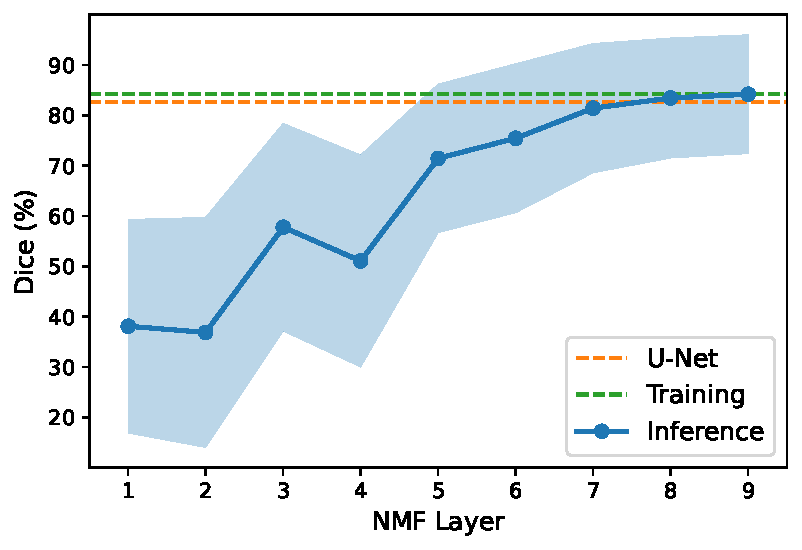
\includegraphics[width=.95\textwidth]{figures/dice_vs_keeptill_swin-factorizer.pdf}
			\caption{}
			\label{fig: dice_vs_keeptill}
		\end{subfigure}%
		\begin{subfigure}{.5\textwidth}
			\centering
			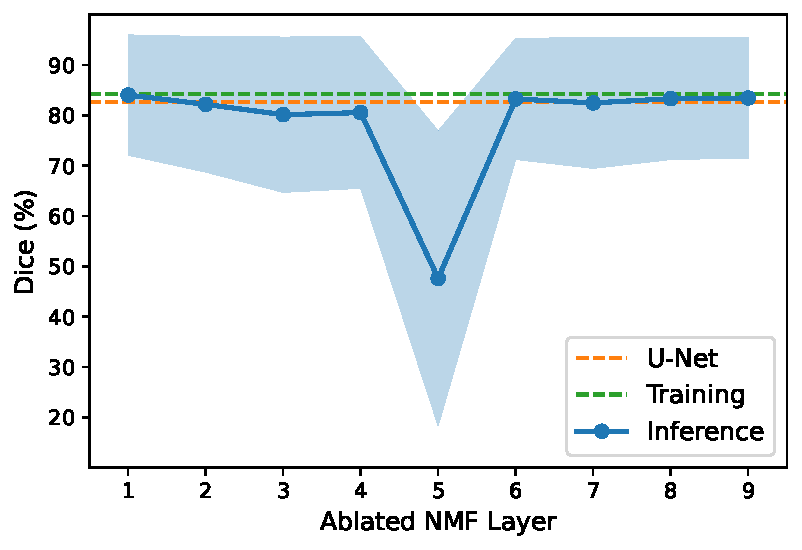
\includegraphics[width=.95\textwidth]{figures/dice_vs_rm_swin-factorizer.pdf}
			\caption{}
			\label{fig: dice_vs_rm}
		\end{subfigure}
		
		\begin{subfigure}{.5\textwidth}
			\centering
			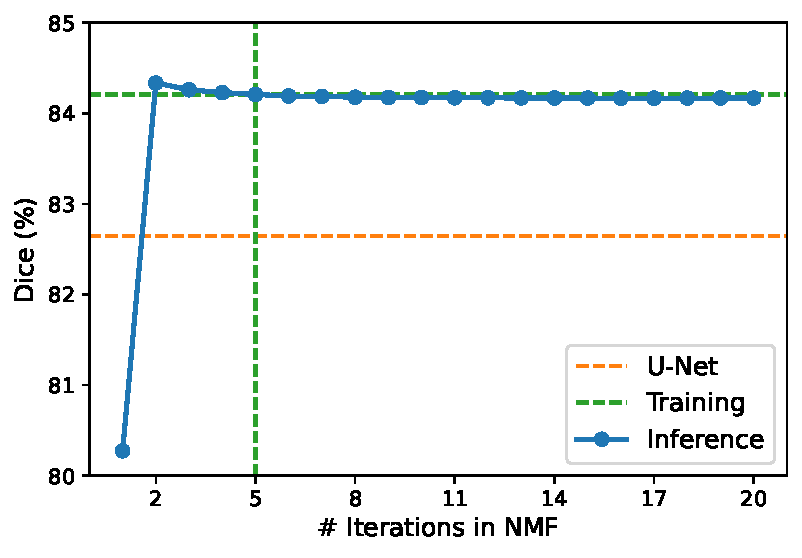
\includegraphics[width=.95\textwidth]{figures/dice_vs_iters_swin-factorizer.pdf}
			\caption{}
			\label{fig: dice_vs_iters}
		\end{subfigure}%
		\begin{subfigure}{.5\textwidth}
			\centering
			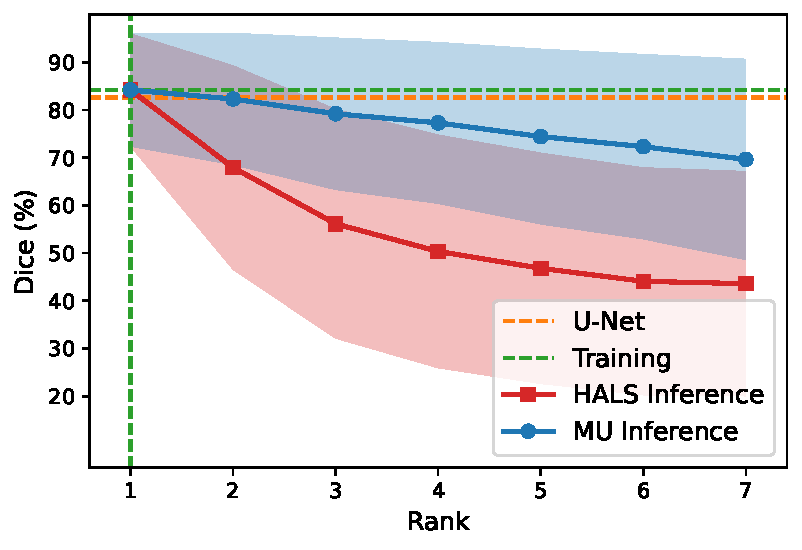
\includegraphics[width=.95\textwidth]{figures/dice_vs_rank_swin-factorizer.pdf}
			\caption{}
			\label{fig: dice_vs_rank}
		\end{subfigure}
		\caption{Inference-phase ablation experiments with Swin Factorizer pre-trained on BraTS. Panel (a) shows the average Dice score when  the first NMF layers are only kept, while Panel (b) shows the Dice score plotted versus the NMF layer removed. Panel (c) shows the plot of Dice against the number of outer iterations in HALS. Panel (d) shows the impact of rank on the performance in HALS and MU. The dashed orange lines indicate the U-Net Dice score, while the dashed green lines correspond to the pre-trained Swin Factorizer model.}
		\label{fig: inference ablation swin factorizer}
	\end{figure} 
	
	
	\paragraph{NMF Solver Iterations.} 
	We investigate the effect of changing the number of outer iterations ($ T $) in HALS. Recall that all the Factorizer models were originally trained using HALS with $ T = 5 $. Figure \ref{fig: dice_vs_iters} shows the results of experimenting with $ T \in \{1, \dots, 20\} $ in the inference phase for the Swin Factorizer model pre-trained with $ T = 5 $. We noticed that for $ T > 1 $, the performance is very close to that of the original model ($ T = 5 $). Interestingly, $ T \in \{2, 3, 4\} $ yielded even higher average Dice scores compared to the original model although the improvement was not statistically significant. We attribute this to the possible regularization effect of reducing $ T $. Note that we proportionally decreased the computational cost of NMF layers by reducing $ T $ while preserving the accuracy. This brings a great advantage to Factorizers over CNNs and Transformers, when it comes to model speed-up (discussed further in Section \ref{sec: discussion}).
	
	
	\paragraph{Rank.} 
	We investigated the impact of changing the rank of the pre-trained Swin Factorizer model in the inference phase. Recall that Swin Factorizers were trained with $ R = 1 $, in which both HALS and MU lead to the same update rule. Therefore, for $ R > 1 $ in inference, we experimented with both HALS and MU in order to make a comparison. In Figure \ref{fig: dice_vs_rank}, the average Dice score on BraTS is plotted as a function of rank. As observed, the more the rank deviated from $ R = 1 $ (the one used in training), the more significantly the Dice score dropped. In comparison to HALS, MU demonstrated a less dramatic reduction in the performance as we increased the rank. This can be due to the fact that within the same number of outer iterations, HALS typically makes a larger decrease in the NMF objective (given in equation \eqref{eq: nmf objective}), causing the HALS-based model to deviate further from the original model than that of MU. 
	
	
	\section{discussion} \label{sec: discussion}
	
	Here, we elaborate on some key features distinguishing Factorizer from other approaches. Similar to self-attention, the Wrapped NMF layer can be viewed as an adaptive filter, meaning that the computation of factor matrices involve the input, as opposed to convolution, where kernel weights are fixed and independent from the input and do not change after training. For Local and Swin Factorizer, we used a large window size of $ (8, 8, 8) $ to aggregate local information, in contrast to typical CNNs comprising $ 3 \times 3 \times 3 $ convolutions. The Wrapped NMF layer scales linearly and is much cheaper than self-attention with quadratic complexity (which is computationally intractable on long sequences) and even Performer, as an efficient approximation of attention. Moreover, by training a Factorizer, we also obtain lightweight yet accurate versions of that for free without needing to re-train any model from scratch. All we need is to reduce $ T $ or ablate some costly NMF layers in the inference phase. As shown in Section \ref{sec: ablation studies}, this did not sacrifice much accuracy on the BraTS dataset and even slightly improved the performance when reducing $ T $ to values greater than 2, probability due to its regularization impact. However, CNNs and Transformers lack such a desirable feature, requiring much more complex mechanisms to achieve their faster versions. 
	
	
	\section{Future Work} \label{sec: future work}
	
	Matrix factorization models are very flexible and versatile. In this work, we used an ordinary NMF model together with some matricization techniques to model local or global context. One possible future work is to customize the NMF objective to simultaneously exploit both local and global contexts. Moreover, it would be useful to explore some ideas for automated selection of the rank hyperparameter, for example, by taking a greedy approach to NMF, a.k.a Nonnegative Matrix Underapproximation, where the components are constructed and added one by one (sequentially) until some criteria are met. This can benefit especially Local Factorizer as different regions happen to have different optimal ranks depending on their contexts. Finally, we will explore the effectiveness of other NMF variants, such as Semi-NMF and Convex-NMF, which work on mixed-signed data matrices and relax the need for the ReLU activation function before factorization.  
	
	
	\section{Conclusion} \label{sec: conclusion}
	
	Vision Transformers, particularly those with hierarchical architectures, have recently achieved results comparable with state-of-the-art CNNs on various computer vision tasks. Nevertheless, lack of locality inductive bias makes them underperform their CNN counterparts in low-data regimes, which is usually the case in medical image segmentation. Moreover, the quadratic complexity of attention makes exiting Transformers apply self-attention layers only after somehow reducing the image resolution, thus fail to fully capture long-range contexts present at higher resolutions. Hence, this paper introduces a series of models, dubbed Factorizer, which leverage the power of low-rank approximation for developing a scalable interpretable approach to context modeling by formulating Nonnegative Matrix Factorization (NMF) as a differentiable layer integrated into an end-to-end U-shaped architecture. Build upon NMF and shifted window idea, Swin Factorizer competed favorably with CNN and Transformer baselines in terms of accuracy and scalability, achieving state-of-the-art results on the BraTS dataset for brain tumor segmentation. Our experiments indicated that NMF components are highly meaningful, which gives a great advantage to Factorizers over CNNs and Transformers in terms of interpretability. Moreover, our ablation studies revealed a distinctive feature of Factorizers that allows the speed-up of inference for a pre-trained Factorizer with no extra steps and without sacrificing much accuracy.
	
	
	\paragraph{Acknowledgements.}
	The research leading to these results has received funding from EU H2020 MSCA-ITN-2018: INtegrating Magnetic Resonance SPectroscopy and Multimodal Imaging for Research and Education in MEDicine (INSPiRE-MED), funded by the European Commission under Grant Agreement \#813120. This research also received funding from the Flemish Government (AI Research Program). Sabine Van Huffel and Pooya Ashtari are affiliated to Leuven.AI - KU Leuven institute for AI, B-3000, Leuven, Belgium. 
	
	
	\appendix
	\section*{Appendix} \label{app: appendix}
	
	\section{Data Augmentation Pipeline} \label{app: data augmentation pipeline}
	The MONAI library \citep{monai2021} was used for data augmentation. The following random transforms were applied on the fly during training in order:
	\begin{enumerate}	
		\item  \textbf{Affine transform}. An affine transform was applied with a probability of 0.15, where the angles of rotation (in degrees) and the scaling factor were drawn from $ \mathcal{U}(-30, 30) $ and $ \mathcal{U}(0.7, 1.3) $, respectively.
		
		\item \textbf{Flip}. All patches were flipped with a probability of 0.5 along each spatial dimension.
		
		\item \textbf{Gaussian Noise}. Each voxel of a patch was independently subject to additive white Gaussian noise with a variance drawn from $ \mathcal{U}(0, 0.1) $. This augmentation was applied with a probability of 0.15. 
		
		\item \textbf{Gaussian Smoothing}. Each modality of a patch was filtered independently via a symmetric Gaussian kernel whose width (in voxels) was drawn from $ \mathcal{U}(0.5, 1.5) $. This augmentation was applied with a probability of 0.15. 
		
		\item \textbf{Scale Intensity}. Voxel intensities were scaled with $ s \sim \mathcal{U}(0.7, 1.3) $ with a probability of 0.15.
		
		\item \textbf{Shift Intensity}. Voxel intensities were shifted with offsets drawn from $ \mathcal{U}(-0.1, 0.1) $ with a probability of 0.15.
		
		\item \textbf{Adjust Contrast}. Gamma correction with $ \gamma \sim \mathcal{U}(0.7, 1.5) $ was applied voxel-wise with a probability of 0.15.
	\end{enumerate}	
	
	
	\section{Matricize Implementation Details} \label{app: matricize implementation details}
	
	Algorithm \ref{alg: local-swin-matricize} presents PyTorch implementations of Local and Swin Matricize modules. Here, we use the \texttt{einops} library to reshape tensors simply by declaring the corresponding Einstein notations.
	
	\begin{algorithm}[t!]
		\caption{PyTorch Pseudocode of Local and Swin Matricize modules. \label{alg: local-swin-matricize}}
		\vspace{5pt}
		\inputminted[fontsize=\footnotesize, linenos]{python}{local-sw-matricize.py}
	\end{algorithm}
	
	
	
	
	\clearpage
	\medskip
	\bibliography{ref}
	
\end{document}